\documentclass[../main/main.tex]{subfiles}
\begin{document}
\dominitoc
\faketableofcontents
\setcounter{chapter}{7}
\chapter{Validation du pipeline
  \hypergal}\label{ch:simu}

\minitoc
\vspace{2cm}
Nous avons présenté et détaillé dans le chapitre précédent le
fonctionnement du pipeline \hypergal. Après s'être assuré de sa
stabilité numérique, nous avons cherché une méthode de validation de son
efficacité. L'objectif est ainsi de quantifier la précision d'extraction
des spectres de supernovae en fonction des conditions d'observation, et
la capacité d'\hypergal\ à les classifier.
Nous avons pour cela choisi de procéder à des simulations de cube
d'observation avec la SEDm.

Dans ce chapitre nous présenterons dans un premier temps la procédure de
génération des simulations, puis nous présenterons les résultats ainsi
obtenus de
l'utilisation d'\hypergal\ sur ces cubes simulés. Nous feront également
pour toutes les analyses une confrontation entre \hypergal\ et la
méthode d'extraction simple, sans modélisation hyperspectral de la
galxie hôte. Nous aurons ainsi une estimation de la robustesse absolue
de notre pipeline, mais également de la robustesse relative avec celui
utilisé par la collaboration ZTF pour la classification des supernovae. 
\newpage

\section{Génération des simulations}\label{sec:simugeneration}

\subsection{Méthode}

Afin de se rapprocher au plus près des conditions d'observation, nous
avons profité de quelques périodes de mise hors service de la caméra
principale ZTF (entre fin novembre 2021 et fin janvier 2022): nous avons ainsi
pu utiliser occasionnellement la SEDm pour observer des galaxies hôtes isolées, dans
lesquelles une supernova a été observée dans le passé.

Nos simulations sont ainsi basées sur une dizaine de ces cubes, extraits
avec l'instrument pour lequel nous souhaitons tester \hypergal, et
contenant dans le champ de vue une galaxie et un fond réels.

Le but est ainsi de rajouter une composante de supernova dans ces
cubes en marginalisant sur les conditions d'observation habituelles
comme le seeing, ou la proportion de chaque type de supernova, tout en explorant
les conditions impactant la robustesse d'\hypergal\ comme la distance
entre la source ponctuelle et le centre galactique, et le rapport signal
sur bruit.

Pour notre étude nous avons créé un jeu de $5000$ cubes de simulations,
et nous  détaillons dans cette section leur conception.

\subsection{Cube de galaxies isolées}
%\label{ssec:xxx}

La base de nos simulations proviennent donc d'observations réelles avec
la SEDm de galaxies ayant accueilli au moins un an dans le passé une
supernova. Ce délai nous permet de nous assurer de l'absence de résidu de l'explosion.
Ces cubes sont donc naturellement dans l'espace de l'instrument pour
lequel \hypergal\ a été conçu.

Les effets d'ADR sont également présents, et il faut donc les
caractériser avant d'inclure une composante de supernova pour que celle
ci soit soumise aux mêmes effets chromatiques. 
Bien que nous connaissons à priori la masse d'air et l'angle
parallactique au début de l'observation, nous ne connaissons pas ces
paramètres effectifs, car ils varient au cours de l'exposition
(de l'ordre d'une demi-heure de temps de pose).

Nous avons pour cela inclu dans \hypergal\ la flexibilité de prendre en
compte ou non n'importe laquelle des composantes de scène, et avons
procéder à l'ajustement de scène avec uniquement la galaxie hôte dans le
MLA. Tout comme détaillé au chapitre précédent, l'ajustement du
centroïde à chaque méta-tranche nous permet d'ajuster les paramètres
effectifs d'ADR. Nos cubes présentent dans notre simulation une masse
d'air allant de $1.01$ à $2.04$, ce qui nous permet de couvrir les
conditions idéales d'observations, les conditions habituelles et les
conditions dégradées.

Nous montrons dans la Figure~\ref{fig:allhostsimu} les cubes intégrés
des galaxies hôtes utilisés pour les simulations, illustrant leur
diversité de morphologie et de position dans le MLA.
\begin{figure}[ht]
  \centering
  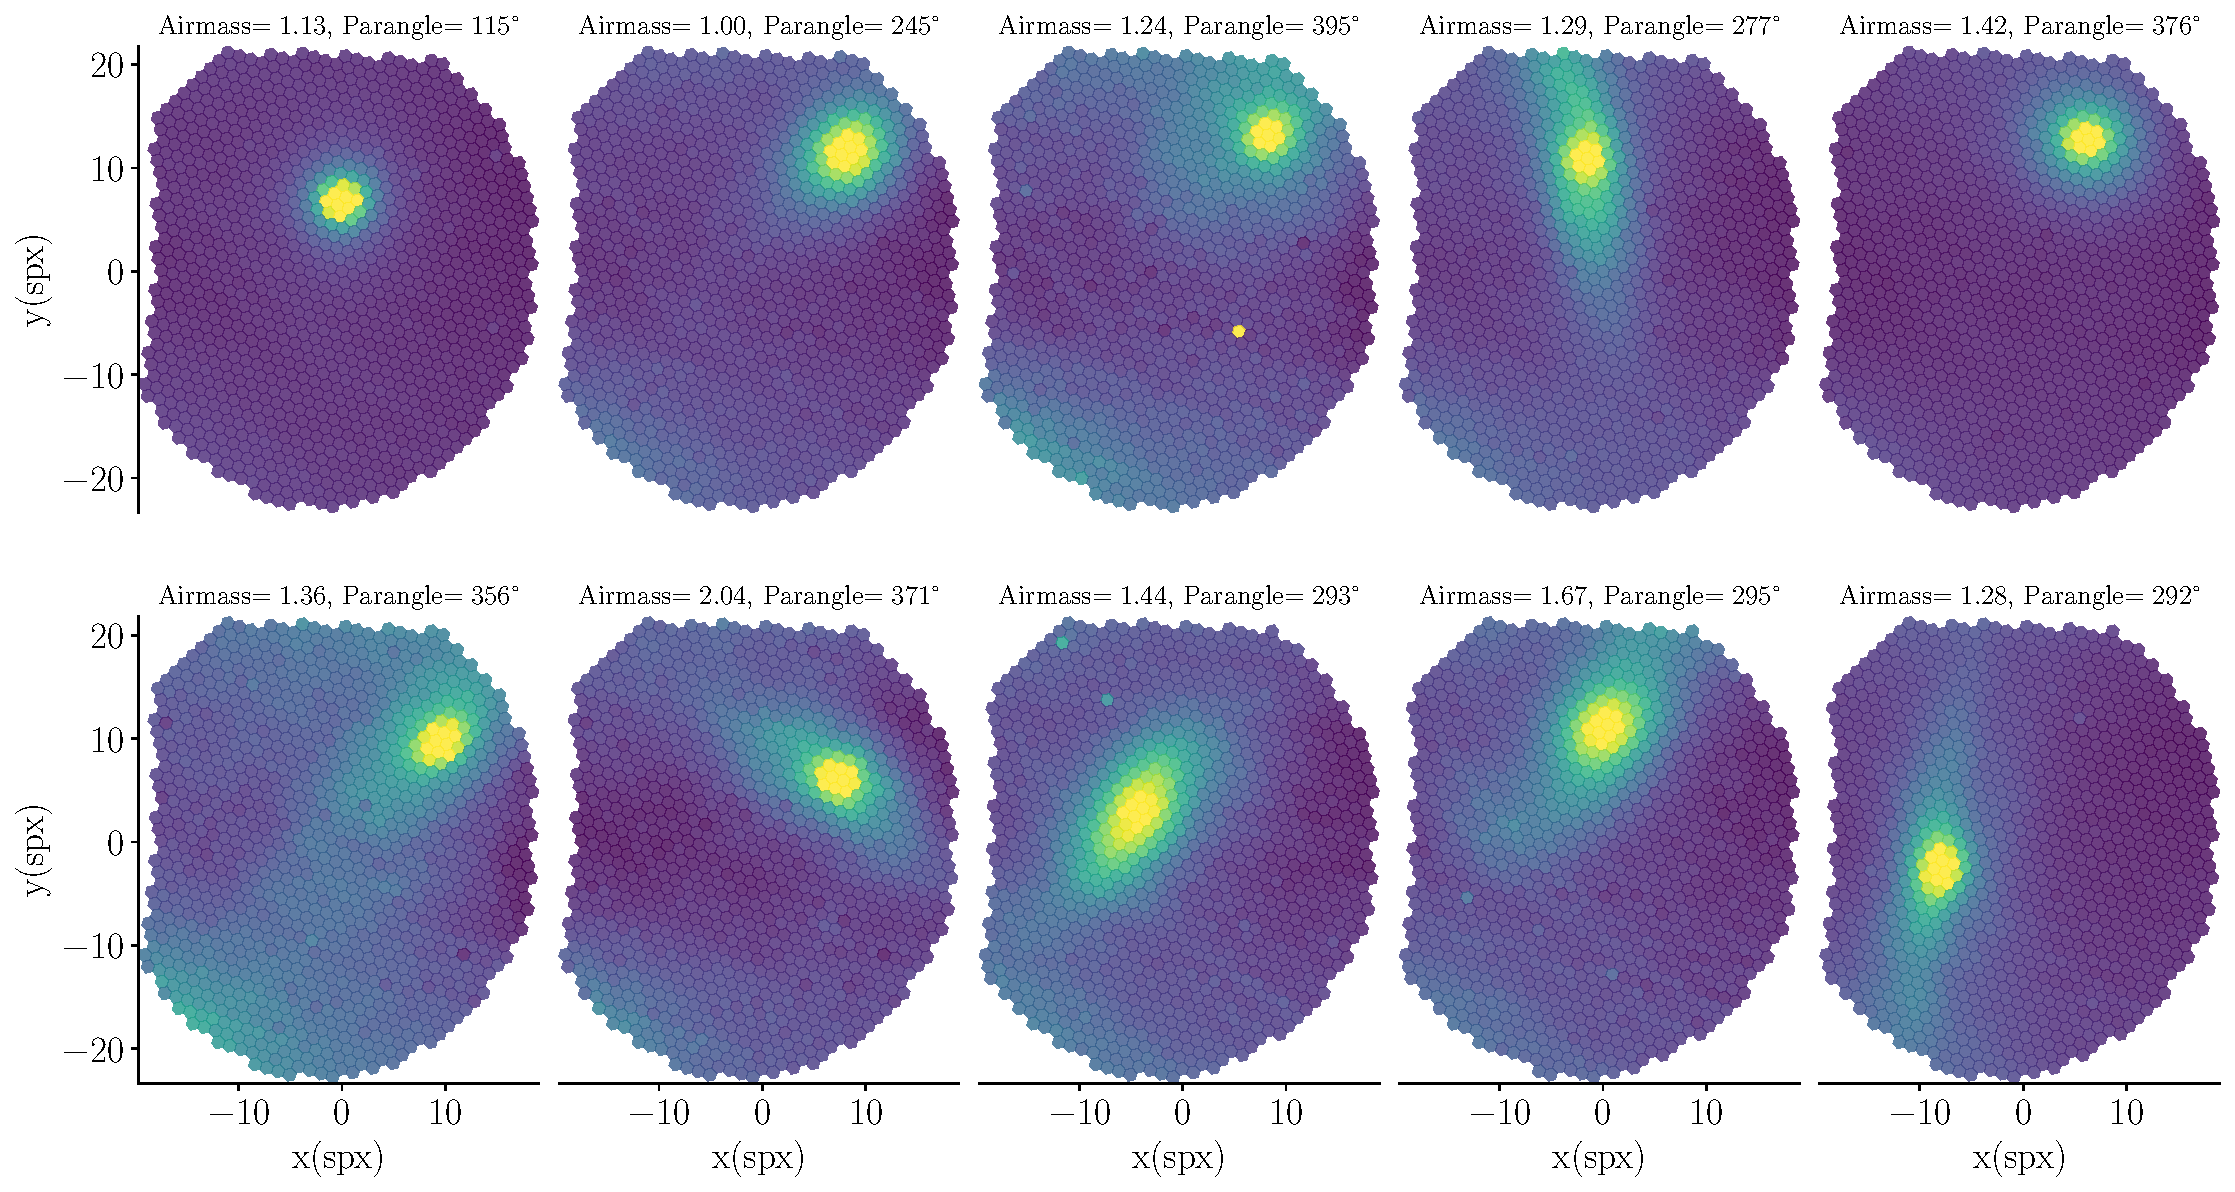
\includegraphics[width=0.99\textwidth]{../figures/08_simu/allhostsimu.pdf}
  \caption[Cubes de galaxies hôtes utilisés pour les simulations.]{Cubes
    intégrés des galaxies hôtes utilisés pour les simulations. Bien que
    nous n'ayons pas eu l'opportunité d'avoir un grand nombre
    d'observations de galaxies isolées avec la SEDm, nous avons fait
    l'hypothèse que ces morphologies et localisations variées de ces
    galaxies étaient suffisamment représentatives des observations pour
    constituer la base des simulations.}
  \label{fig:allhostsimu}
\end{figure}

\subsection{Modèles de supernovae}
% \label{ssec:xxx}

Afin de tester la précision d'extraction de spectre avec \hypergal, il nous faut inclure dans les cubes une source ponctuelle dont le
spectre est connu a priori. L'étude seule de la précision d'extraction
(par exemple avec un RMS spectral) est indépendante de la forme du spectre, et donc du type
de la supernova.
Cependant nous souhaitons également avoir une
estimation de l'efficacité d'\hypergal\ à classifier les supernovae.
Pour analyser ces deux aspects (précision et classification), il faut
donc que le spectre de la source ponctuelle simulée soit connu a priori et que nous connaissions sa classification.

Par manque de temps et afin d'éviter de devoir générer des spectres avec
des outils inconnus, puis les projeter dans l'espace des observations de
la SEDm (transmission, LSF, échantillonnage ...), nous avons choisi
d'utiliser des spectres de supernovae déjà obtenus avec la SEDm, et
classifiés avec SNID.

Afin de s'assurer de la classification, nous n'avons sélectionné que des
spectres avec un très haut r$lap$ (paramètre de qualité/confiance de SNID considéré
comme bon si r$lap>5$, voir section 6.1 de \citet{BlondinSNID}). Pour
les spectres de supernovae de type Ia (les plus nombreuses à être observées), nous avons
sélectionné $70$ spectres avec un r$lap>25$ pour le meilleur modèle, et un r$lap>15$ pour les 30 premiers modèles.

Sur un raisonnement similaire, nous avons sélectionné $7$ spectres de
supernova de type II avec un r$lap>12$. Pour les types Ic et Ib, plus
rarement observés ($\approx5\%$ des observations), nous avons préféré
prendre seulement $1$ spectre de chaque mais avec une très forte
confiance de classification ( r$lap\approx18$ pour la Ib et r$lap\approx15$
pour la Ic).

Nous procédons ensuite sur chacun de ces spectre à un lissage en
appliquant un filtre de Savitzky-Golay \citep{SavitzkyGolay}. Afin de ne pas casser les
structures des spectres, nous utilisons un lissage léger avec un
polynôme d'ordre 3 sur une fenêtre de 5 pixels spectraux.

Nous montrons dans la Figure~\ref{fig:specsimueach} un exemple de
spectre après lissage pour chaque type de supernova, ainsi que le
meilleur modèle de classification SNID et le r$lap$ associé.

\begin{figure}[ht]
  \centering
  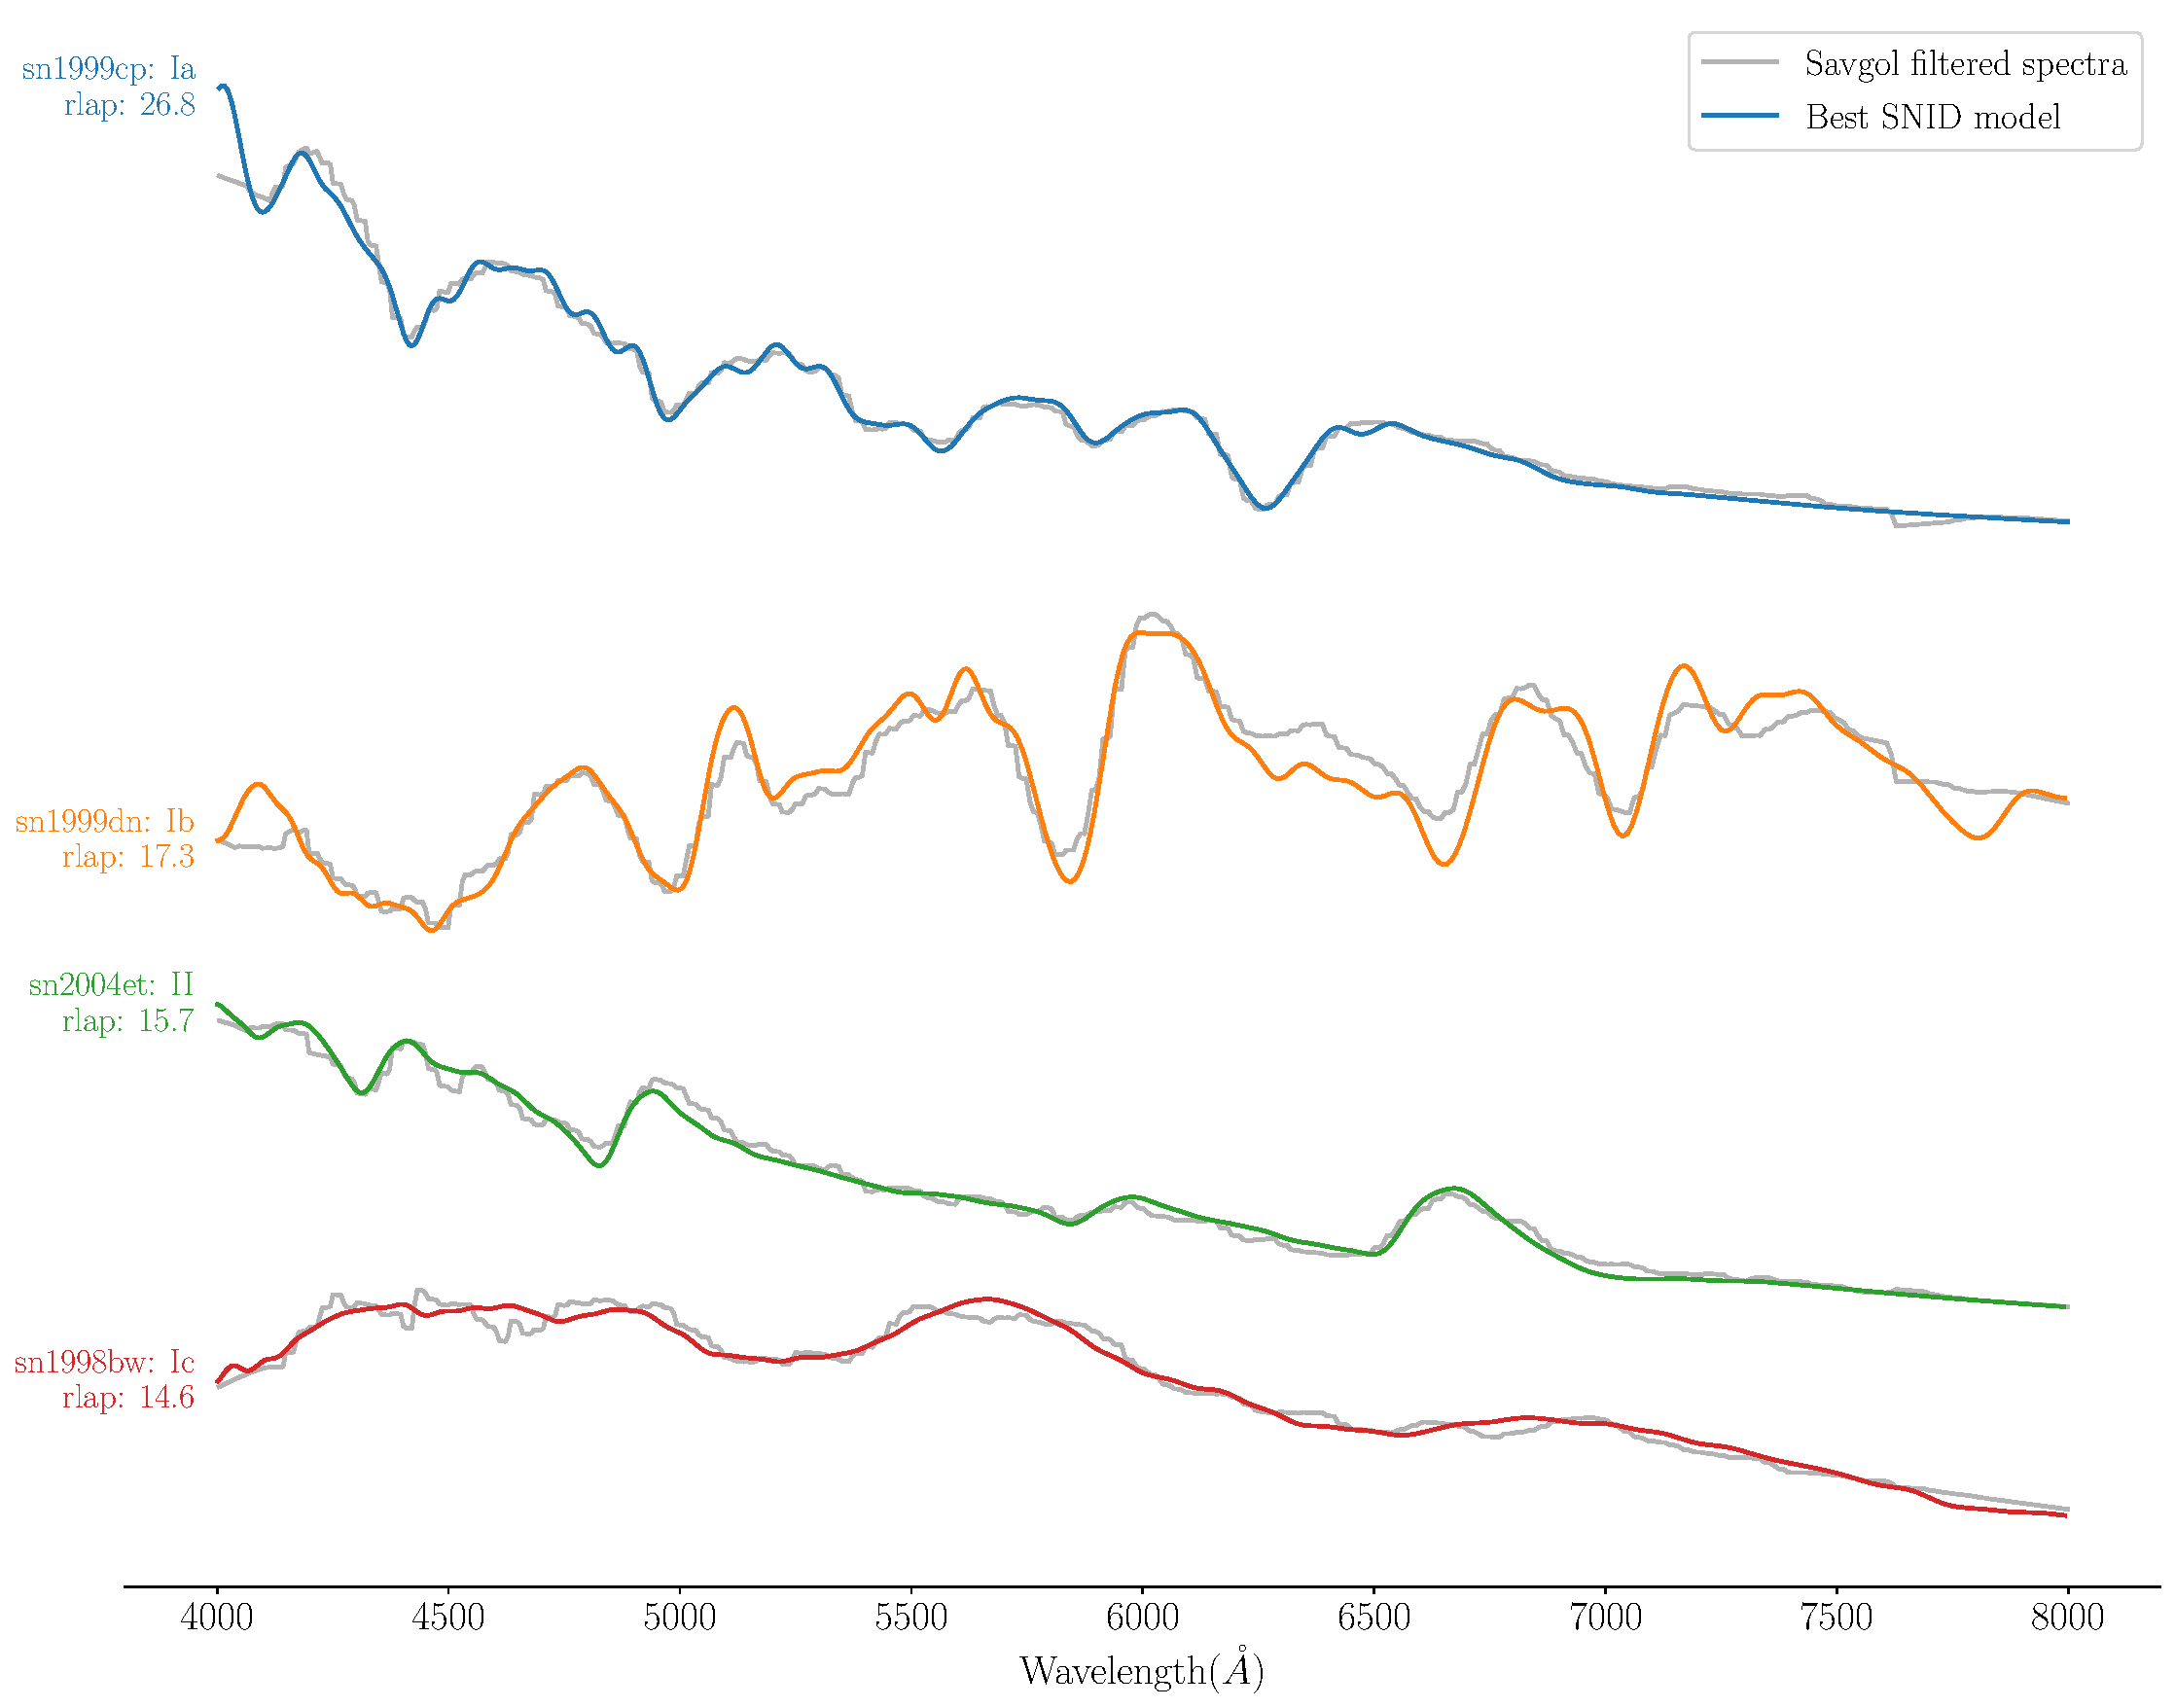
\includegraphics[width=0.99\textwidth]{../figures/08_simu/specsimueach.pdf}
  \caption[Exemple de spectre pour chaque type de supernova pour les
  simulations.]{Exemple de spectre pour chaque type de supernova pour
    les simulations. Nous y montrons en gris le spectre après
    lissage par un filtre de Savitzky-Golay, qui provient d'une
    observation de la SEDm. En couleur nous montrons le meilleur
  modèle de classification SNID et le r$lap$ associé, avec de haut en bas: une SNIa, une
  SNIb, une SNII, et une SNIc.}
  \label{fig:specsimueach}
\end{figure}

\subsection{Marginalisations et paramètres d'étude}
% \label{ssec:xxx}

\subsubsection{Types et phases}

Dans le but de représenter dans nos simulations les proportions
observées de chaque
type de supernova, nous utilisons les statistiques de la Data
Release 1 du groupe Bright Transient Survey de ZTF
\citep[BTS;][]{FremlingZTFspec2020}.
Nous choisissons ainsi de répartir dans nos simulations $80\%$ de SNIae,
$15\%$ de SNeII, $2.5\%$ de SNeIb et $2.5\%$ de SNeIc. Ces deux derniers
types sont habituellement regroupés, nous considèrerons donc par la
suite un groupe de $5\%$ de SNeIbc.

Nous choisissons également de 
procéder à une marginalisation des phases des spectres de SNIea, en se
basant sur les statistiques de la
DR1 du groupe SNeIa de ZTF \citep{DhawanZTFDR1}. Pour
les 70 spectres utilisés, nous déduisons la phase en comparant le
jour d'observation de la supernova dont est issu le spectre avec le pic
de luminosité ajusté par ZTF avec SALT2
\citep{Guysalt2005,Guysalt22007,Guy2010,Betoule2014} sur la courbe de
lumière.

La distribution de phase de notre échantillon s'étend de -15 à
+15 jours, avec une médiane à -2 jours. Nous pouvons ainsi sélectionner
aléatoirement les spectres de SNIa, sachant leur phase et suivant une
distribution équivalente à celle relevée dans \citep{DhawanZTFDR1}. Nous marginalisons nos simulations suivant
une distribution de phase gaussienne, centrée sur $-3$ jours et d'écart
type $4$ jours.

\subsubsection{Seeing}

Les supernovae étant des sources ponctuelles à ajouter dans nos cubes
de simulations, elles sont entièrement caractérisées par leur profil de
PSF.

Nous faisons l'hypothèse d'un profil connu a priori, et
utilisons le profil radial développé au chapitre~\ref{ch:irf} avec
l'étude des étoiles standards. Afin de représenter une distribution en
seeing similaire à celle observée par la SEDm, nous marginalisons nos
simulations sur le seeing en utilisant les
distributions conjointes des paramètres de forme de PSF ajustés des $2202$
étoiles standards extraites pour l'étude de la calibration en
flux (section~\ref{sec:validationpsf}).

Nous faisons donc la supposition que la distribution en seeing des
étoiles standards est représentative de celle des supernovae. Bien que
la contribution de l'optique du télescope soit indépendante
de l'objet observé, il faut noter que les étoiles standard le sont
habituellement avec une masse d'air comprise entre $1$ et
$1.2$. Nos simulations ayant une masse d'air comprise entre $1$ et $2$, cela implique potentiellement une sous-estimation que nous
n'avons pas caractérisé de la
distribution en seeing utilisée pour nos simulations.

\subsubsection{Distance supernova/centre galactique}\label{ssec:distancesimu}

\hypergal\ a été conçu pour répondre à la problématique de la
contamination par la galaxie hôte. Nous voulons donc explorer la
précision d'extraction de spectre des SNe et l'efficacité de
classification suivant la distance séparant la source ponctuelle du
cente galactique. Dans ces simulations nous ne nous intéressons pas aux
cas où la supernova est complètement isolée dans le champ de vue, ayant
déjà entrainé le pipeline avec les étoiles standards.

Nous utilisons une distribution uniforme comprise entre $0$ et $10$
spaxels de distance, ce qui correspond à un intervalle entre $0$ et
$\approx5\farcs6$. Cette distance seuil représente généralement environ $2$ à $3$ largeur à
mi-hauteur suivant le profil radial des sources ponctuelles, ce qui nous
semble suffisant pour explorer un large intervalle de séparation
angulaire jusqu'à la limite d'une isolation totale de la supernova.

Nous prenons également en compte que lors des observations réelles, les
supernovae sont habituellements situées vers le centre du MLA. Ainsi
afin d'éviter de simuler une cible dans un des coins du cube, nous
restreignons la localisation possible de la source ponctuelle dans un
disque de $12$ spaxels de rayon au centre du MLA. Pour les cas où la
galaxie est très excentrée et que nous simulons une source ponctuelle
proche du centre galactique, nous privilégions de la positionner dans le
quart de cercle en direction du centre du MLA. 

\subsubsection{Constraste}

Le dernier paramètre que nous utilisons pour explorer la robustesse
d'\hypergal\ correspond à l'intensité du flux de la supernova par
rapport à ce qui se situe à sa localisation: nous introduisons ainsi le
contraste $c_{r}$, défini dans la bande photométrique équivalente $ZTF_{r}$
afin de pouvoir plus aisément comparer les résultats des simulations
avec un cas réel d'observation, exprimé comme:
\begin{equation}
  \label{eq:contrast}
  c_{r} = \frac{S_{r}}{S_{r}+B_{r}}
\end{equation}
avec $S_{r}$ le signal de la supernova et $B_{r}$ le signal de tout ce qui se
situe en fond (ciel + galaxie).

Afin de déterminer la quantité $B_{r}$ qui contamine le signal de la
supernova, il faut prendre en compte le profil de PSF utilisé pour
simuler la source ponctuelle. En effet, si on suppose que la SN est
centrée (pour une longueur d'onde donnée) à la position ($x_{0}$,
$y_{0}$), alors le signal de fond à la même position aura un plus grand
impact de contamination que le fond à la position ($x_{0}+\d x_{0}$,
$y_{0}+\d y_{0}$).

Pour prendre cela en compte et plutôt que de considérer une ouverture fixe
autour de la localisation de la SN simulée pour définir $B_{r}$, nous
multiplions le cube de simulation sans la SN par un cube ne contenant
que le profil de PSF (normalisé avec un pic à $1$) à la localisation de
simulation de la SN.

Le contraste est ainsi défini dans l'intervalle $]0,1[$, $0$ impliquant
que la supernova n'existe pas, et $1$ qu'elle est infiniment plus
intense que le fond (ou que le fond est à zéro ce qui n'est pas notre
cas ici).

Nous pouvons également relier le contraste au rapport $R=\frac{S_{r}}{B_{r}}$:
\begin{equation}
  \label{eq:rapportSB}
  c_{r} = \frac{R}{1+R}
\end{equation}

Les simulations sont ainsi générées suivant une distribution uniforme du
contraste $c_{r}$ entre $0$ et $1$.

Nous pouvons également voir que le rapport signal sur bruit est
étroitement lié au contraste. En effet, en supposant que le signal dans
le cube est
entièrement caractérisée par une loi de Poisson, nous avons alors que:

\begin{equation}
  \label{eq:SNR}
  SNR_{r} \triangleq \frac{S_{r}}{\sqrt{\sigma_{S_{r}}^{2}+\sigma_{B_{r}}^{2}}}\approx
  \frac{S_{r}}{\sqrt{S_{r}+B_{r}}} = c_{r}\times\sqrt{S_{r}+B_{r}}
\end{equation}
avec $S_{r}$ et $B_{r}$ en unités de coups. Avec un raisonnement similaire nous
pouvons montrer que:
\begin{equation}
  \label{eq:logsnr}
  SNR_{r}\approx R\times\sqrt{B_{r}} = \frac{C_{r}}{1-C_{r}}\times\sqrt{B_{r}}
\end{equation} 

En pratique, nous sommes en mesure de récupérer la quantité
$\sigma_{B}$, car présente dans le cube SEDm avec la galaxie hôte
isolée. Pour remonter au SNR, nous utilisons directement sa définition
en supposant que le bruit à ajouter dans le cube à cause du signal de la
supernova simulée est $\sigma_{S}^{2}=S$.

\subsection{Création des cubes de simulation}

Après avoir procéder à la marginalisation des proportions de chaque type
de supernova, de la phase des Ia et du seeing, nous générons un jeu de
$N\times m$ paramètres avec $N$ le nombre de simulations (5000), et $m$
les paramètres de la simulation:\\

\begin{itemize}[label=$\diamondsuit$]
  \itemsep0em
 \begin{samepage}
\item Cube de la galaxie hôte;
\item Spectre de supernova;
\item Paramètres de PSF décrivant la SN;
\item Distance entre la SN et le centre galactique;
\item  Contraste.
  \end{samepage}
\end{itemize}

Pour pouvoir ajouter le signal de la supernova simulée et surtout le
bruit associé, nous devons utiliser le cube SEDm en unité de flux
ADU et travailler dans ces unités avec le spectre de la SN.
Connaissant a priori la calibration en flux qui sera utilisé pour chacun des
cubes, nous appliquons une calibration inverse sur le spectre à simuler,
qui est initialement en unité de flux physique.

La création d'un cube de simulation sachant les $m$ paramètres se fait ensuite en plusieurs étapes:

\begin{minipage}{\textwidth}%
  \begin{enumerate}[(a)]
    \itemsep=0em
    \item \textbf{Détermination de la localisation ($x_{ref}$, $y_{ref}$) de la supernova} dans le cube
      à une longueur d'onde de référence ($\lambda_{ref}=6000$\AA):
      nous prenons aléatoirement une position sur le cercle centré sur
      la galaxie, avec un rayon égal à la distance simulée
      SN/galaxie. Nous prenons en compte les contraintes pour éviter les
      bords du cube expliquées dans la section~\ref{ssec:distancesimu};
      
  \item \textbf{Détermination du signal de fond $B$:} nous construisons un cube vide dans
    lequel nous plaçons le profil de PSF à la localisation et longueur
    d'onde fixée à l'étape
    précédente. La localisation est propagée pour toutes les tranches
    avec le modèle d'ADR, sachant les paramètres de masse d'air et
    d'angle parallactique, et le profil est normalisé à un pic égal à $1$ pour chaque
    longueur d'onde. Nous multiplions alors le cube de galaxie par
    celui-ci, le résultat étant un cube contenant uniquement le signal de fond $B$
    contaminant la SN.

  \item \textbf{Détermination du coefficient multiplicatif à appliquer sur le
    spectre de la supernova.} Nous déterminons grâce à l'étape précédente le fond contaminant $B_{r}$
    dans la bande équivalente $R$ de ZTF. Connaissant également le spectre de la
    supernova en ADU, nous en déduisons son signal $S'_{r}$ dans
    la bande $R$ avant adaptation au
    contraste souhaité. Enfin, connaissant $B_{r}$, $S'_{r}$ et $c_{r}$, nous
    appliquons le
    coefficient multiplicatif nécessaire sur l'ensemble du spectre de la
    SN (et donc sur $S'_{r}$) pour obtenir le constraste souhaité.

   \item \textbf{Ajout du bruit associé à la supernova.} Nous supposons que le
     flux ajouté de la supernova simulée est entièrement caractérisé
     par une loi de Poisson, et ajoutons donc au cube SEDm pour chaque
     spaxel de chaque tranche une variance telle que $\sigma_{S,\lambda,spx}^{2}=S_{\lambda,spx}$.

   \item \textbf{Détermination du SNR.} Le SNR n'est pas un paramètre de
     nos simulations, mais nous pouvons le récupérer et le stocker connaissant
     $B_{r}$, $S_{r}$, $\sigma_{B_{r}}$ et  $\sigma_{S_{r}}$.

   \item \textbf{Construction du cube de simulation}. Tous les
     ingrédients sont réunis pour la construction du cube: le spectre de
     la supernova, sa position chromatique, son profil de PSF
     chromatique et le coefficient multiplicatif pour avoir le contraste désiré.
  \end{enumerate}
\end{minipage}\\


Nous procédons ainsi à la générations des $5000$ cubes de
simulations. Dans la Figure~\ref{fig:examplesimu} nous illustrons
quelques exemples de ces cubes pour différentes valeurs de contraste,
distance, type de SN et SNR.
\begin{figure}[ht]
  \centering
  \makebox[\textwidth][c]{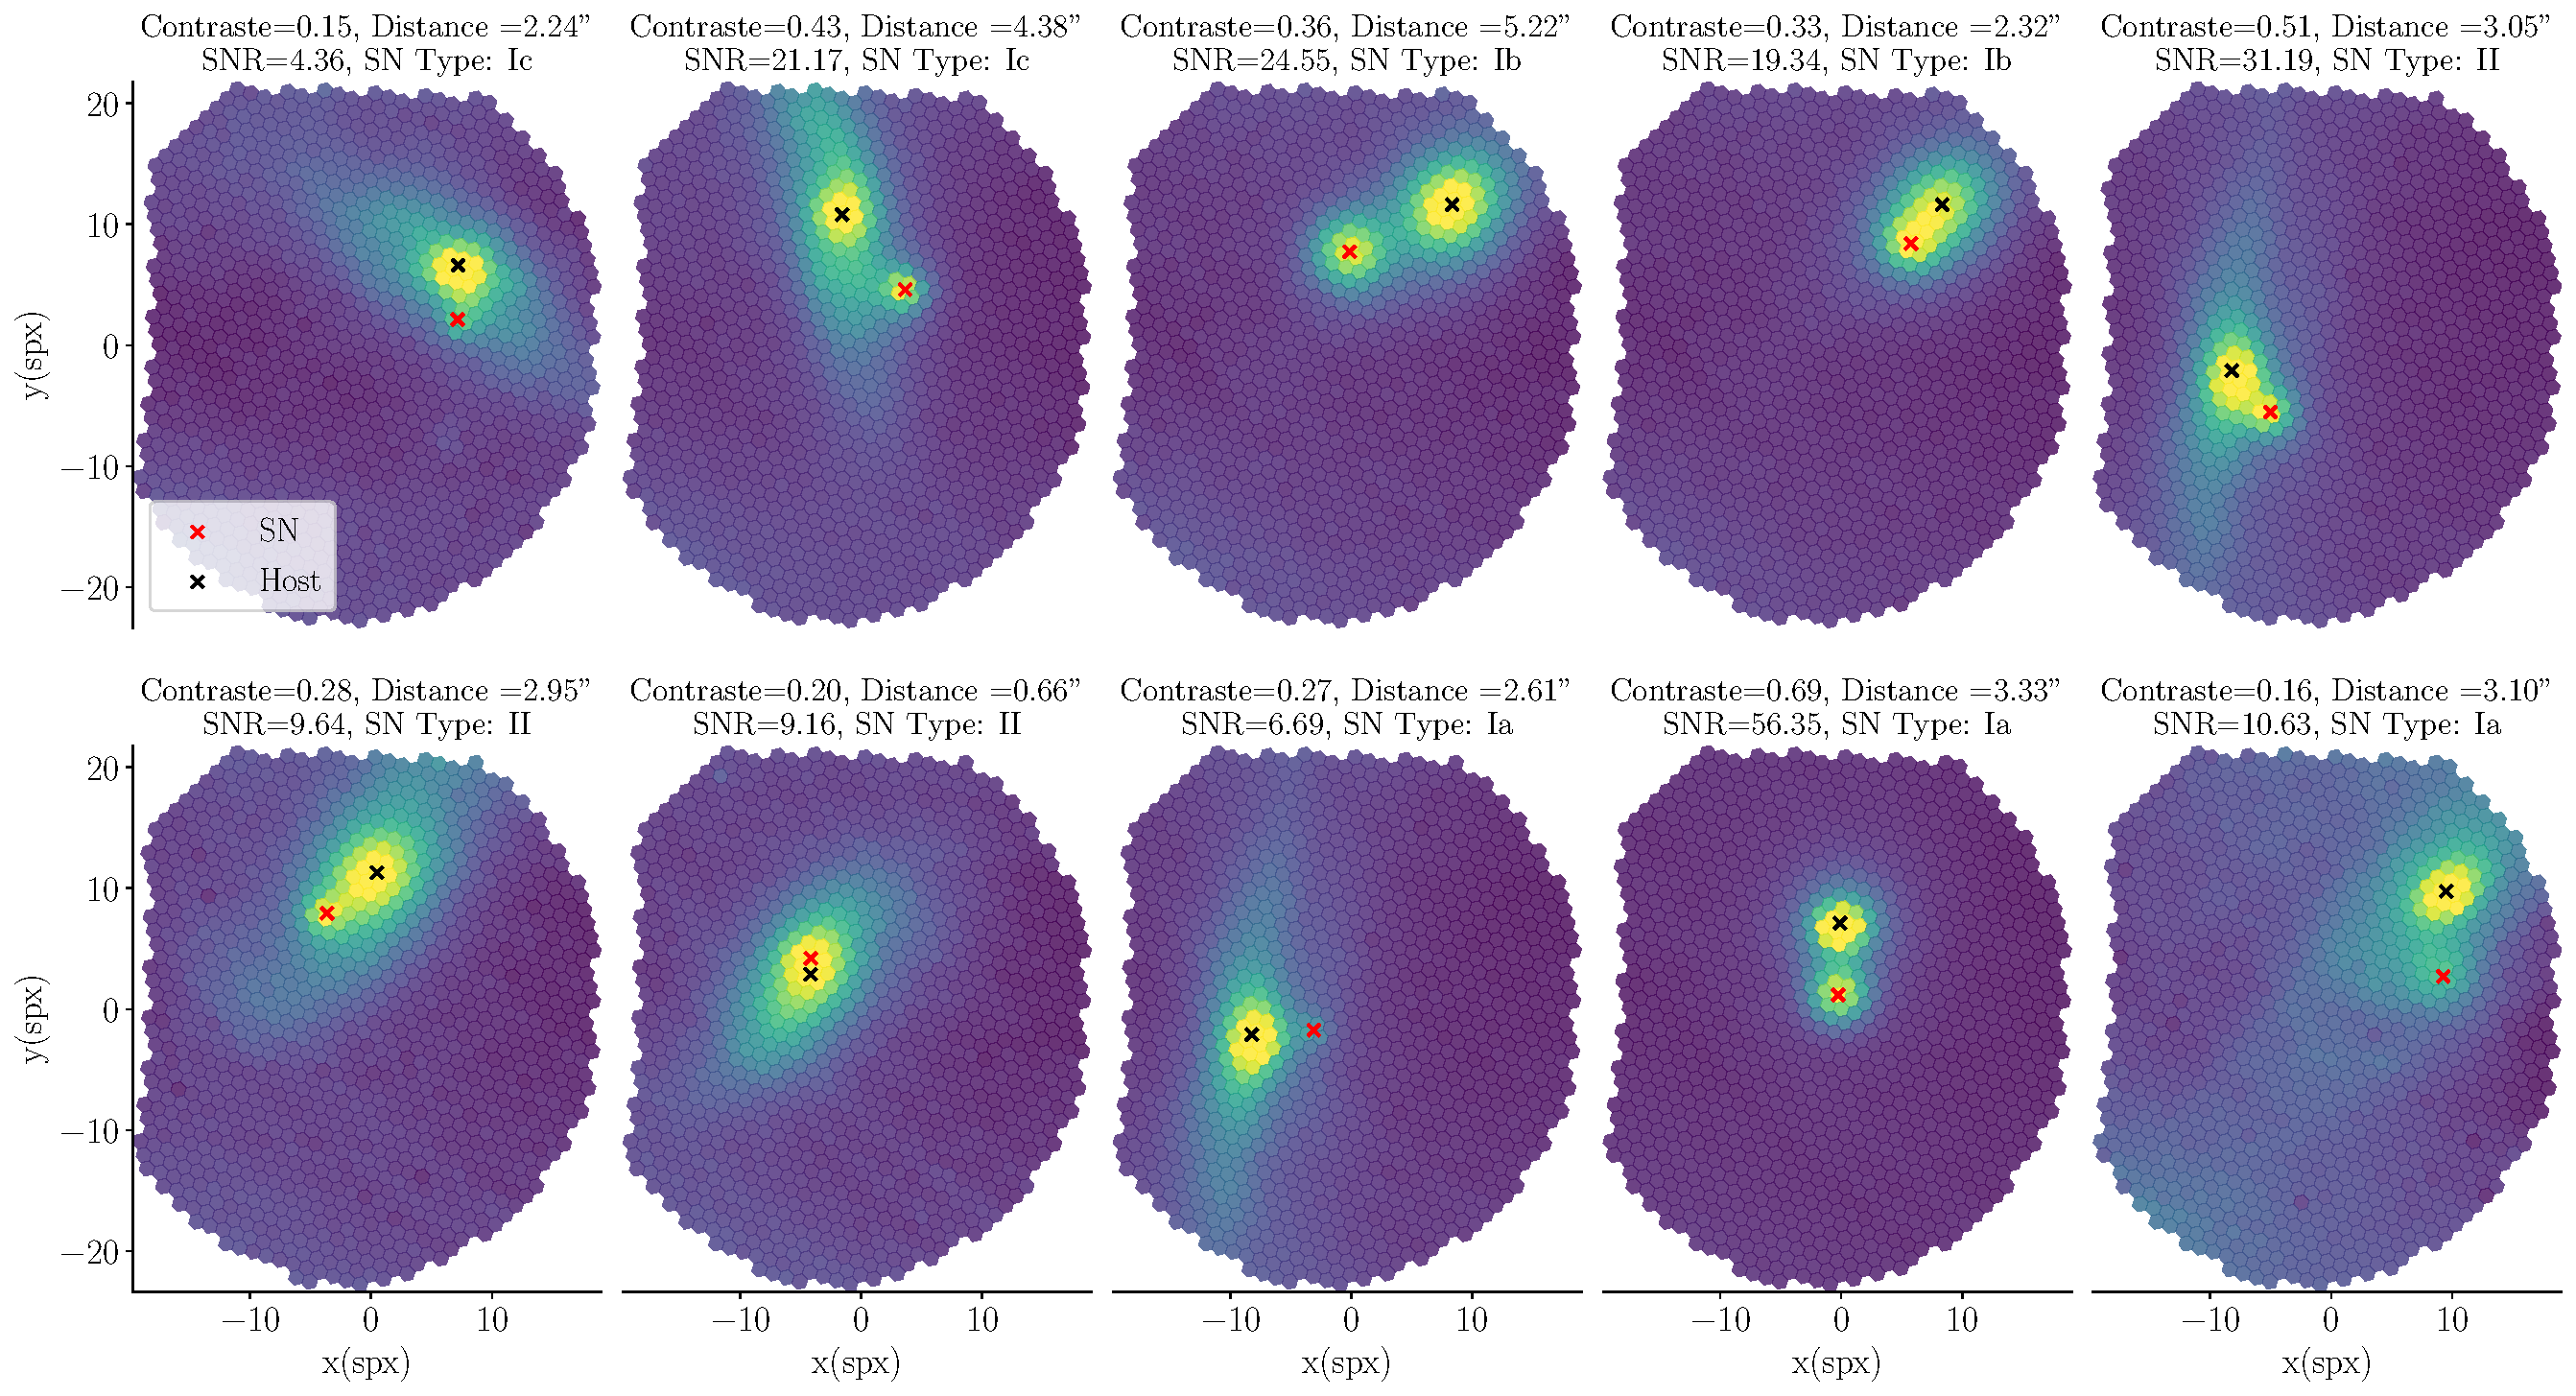
\includegraphics[width=1.15\textwidth]{../figures/08_simu/examplesimu.pdf}}%
  \caption[Examples de cubes de simulation.]{Examples de cubes de
    simulation pour différentes valeurs de contraste, distance, type de
    SN et SNR.}
  \label{fig:examplesimu}
\end{figure}

\section{Résultats et précision}\label{sec:simuresult}

Après avoir généré nos cubes de simulation, nous avons fait tourner
\hypergal\ suivant 2 méthodes: la première avec une modélisation de
scène comprenant toutes les composantes comme détaillée au chapitre
précédent. Et une deuxième fois avec la même méthode d'extraction que le
pipeline d'origine \pysedm, sans modélisation de la galaxie hôte.

Nous n'avons pas utilisé directement le pipeline \pysedm\ car les modèles
de PSF et de fond sont différents de celui d'\hypergal, ce qui n'aurait
pas permis une comparaison robuste. La méthode d'extraction est cela dit
identique, suivant le procédé détaillé dans \citet{pysedm} et la section~\ref{ssec:sourceextractpysedm}.
Les seules différences avec la modélisation de scène complète étant
l'absence de modèle de galaxie, et le fait que l'on ne considère qu'un
disque de $10$ spaxels de rayon autour de la position de la supernova
pour son extraction.

En plus d'une étude de la robustesse absolue d'\hypergal, cette
confrontation nous permet d'avoir également une idée de l'amélioration
apportée avec ce nouvel outil d'extraction de spectre.

Nous dénominerons dans la suite du manuscrit l'indice $_{HG}$ pour la
méthode de modélisation de scène \hypergal, et $_{PS}$ pour la méthode
d'extraction de source ponctuelle basique.

Dans cette section nous allons étudier 3 informations pour chacune des 2
méthodes:

\begin{itemize}[label=$\diamondsuit$]
  \itemsep0em
 \begin{samepage}
\item \textbf{La précision spectrophotométrique}, c'est à dire une
  comparaison brute du spectre de simulation et du spectre extrait;
\item \textbf{La précision après correction du continuum}, à l'instar de
  la méthode de pré-traitement utilisé dans \pkg{SNID}
  (section~\ref{sec:snid}). La SEDm ayant été conçu pour la
  classification de spectres, ce qui nous importe est la
  capacité d'\hypergal\ à extraire les informations spectrales
  permettant cette classification, c'est à dire la structure du spectre
  traduisant les caractéristiques de tel ou tel type.
\item \textbf{L'efficacité de classification}. Pour cela nous
  utiliserons le même classifieur utilisé par ZTF, \pkg{SNID}, et nous
  comparerons la classification du spectre extrait avec celui connu a priori.
  \end{samepage}
\end{itemize}

Plutôt que d'utiliser le contraste comme paramètre d'étude, nous
utiliserons le rapport signal sur bruit. Comme introduit dans
l'équation~\ref{eq:logsnr}, le SNR est étroitement lié au
contraste car linéairement proportionnel au rapport $R=S_{r}/B_{r}$. Nous illustrons cette corrélation dans la
Figure~\ref{fig:corr_SNR_contrast}, montrons la relation linéaire entre
le SNR et la quantité $R=\frac{C_{r}}{1-C_{r}}$.

\begin{figure}[ht]
  \centering
  \makebox[\textwidth][c]{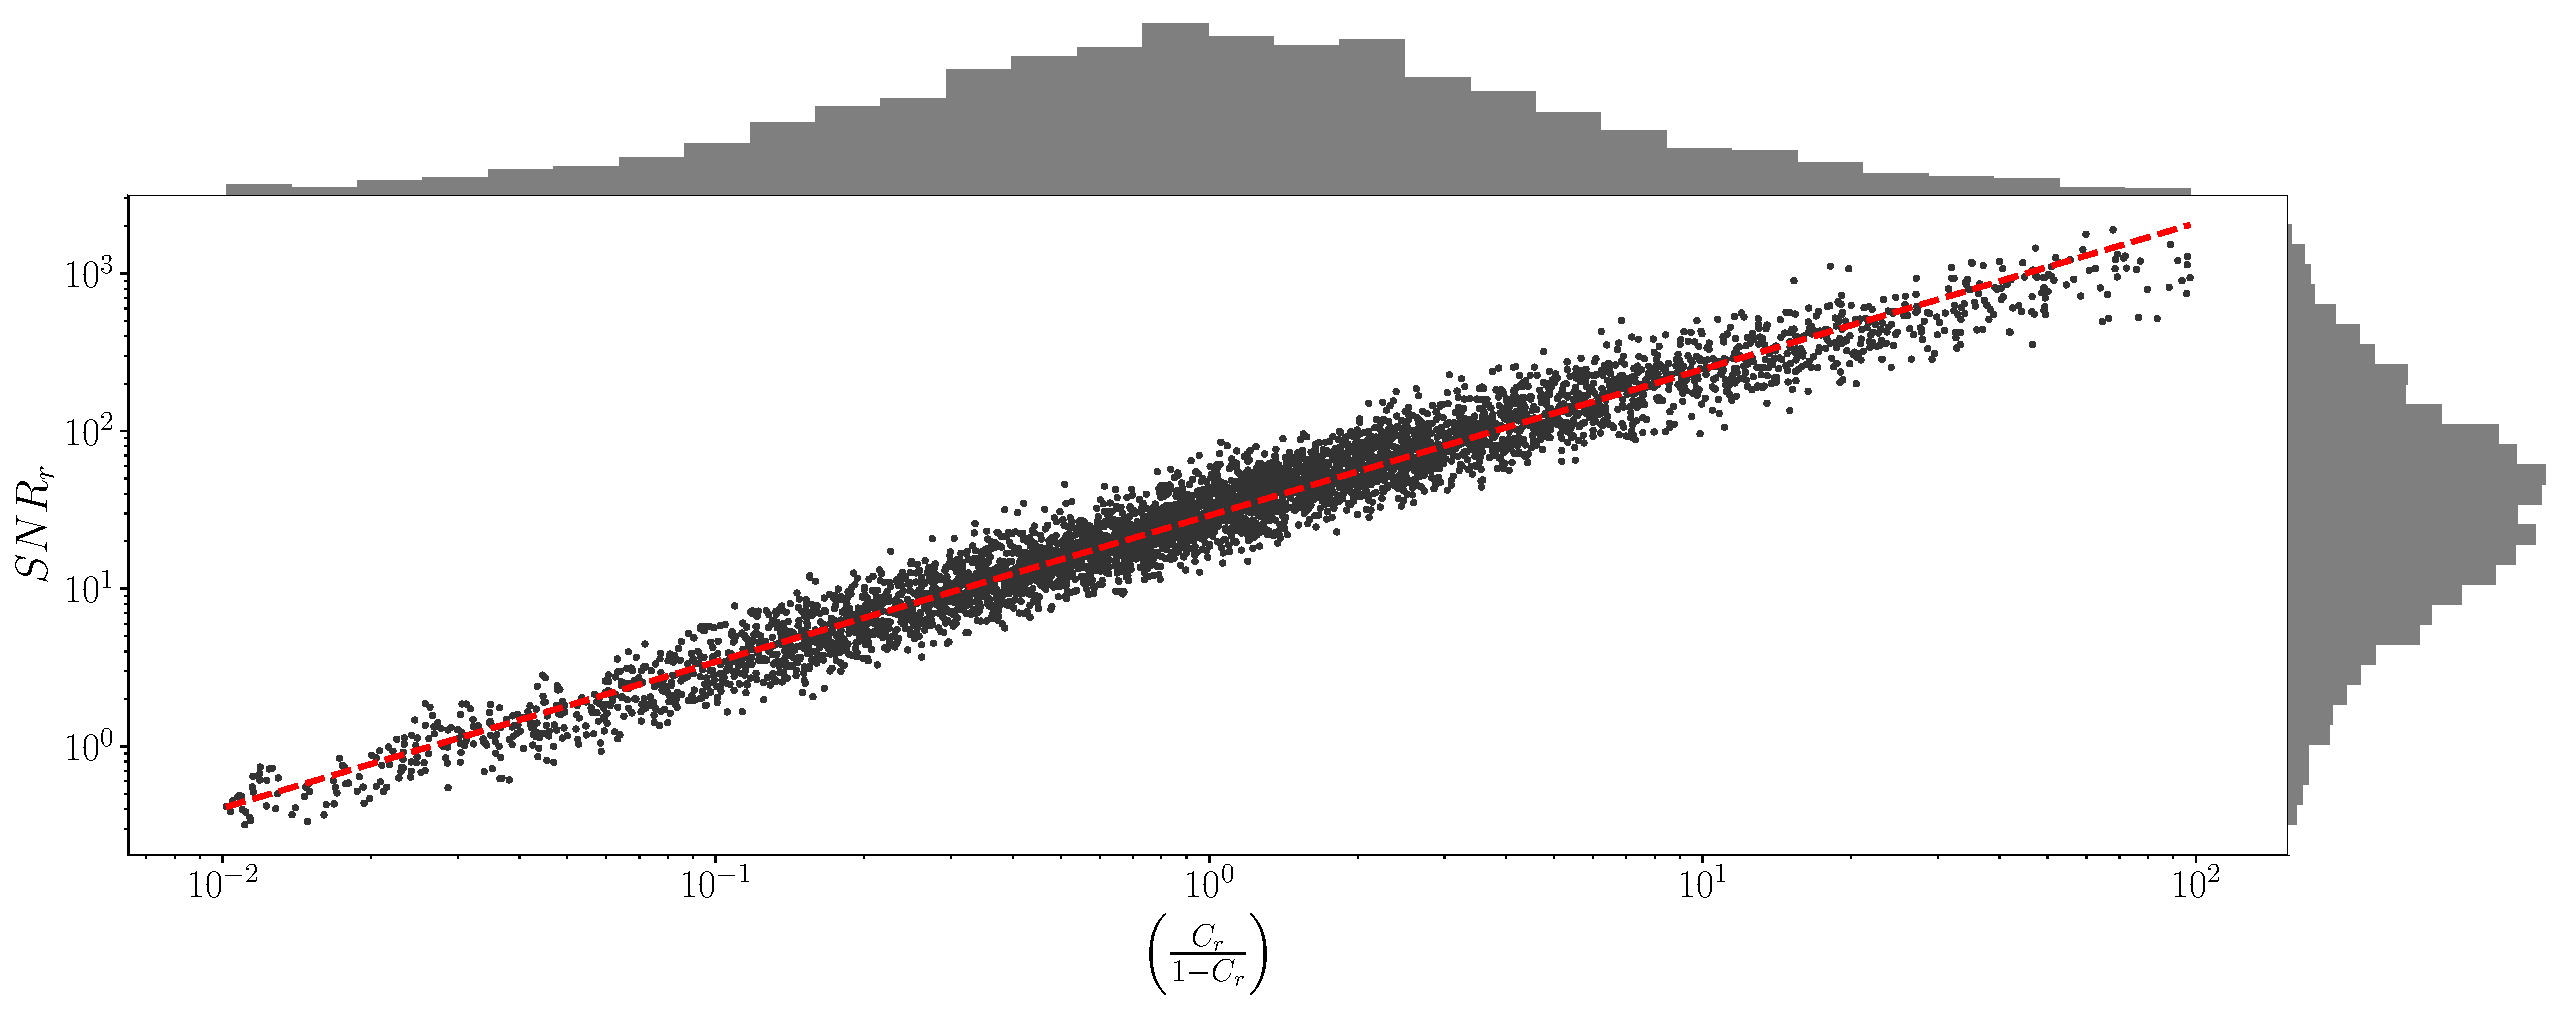
\includegraphics[width=1.\textwidth]{../figures/08_simu/corr_SNR_contrast.pdf}}%
  \caption[Corrélation SNR/contraste des simulations.]{Corrélation
    SNR/contraste des simulations et leur distribution respective. Nous
    montrons dans cette figure en échelle logarithmique le rapport signal
    sur bruit en fonction de la quantité $R=\frac{C_{r}}{1-C_{r}}$,
    introduite dans l'équation~\ref{eq:logsnr}. La
    droite en pointillés rouge indique la régression
    linéaire, et la dispersion autour de celle ci provient de la
    contribution du fond, $\sqrt{B_{r}}$, propre à chaque simulation.}
  \label{fig:corr_SNR_contrast}
\end{figure}

\subsection{Précision spectrophotométrique}\label{ssec:spectrophotoaccuracy}

Commençons par étudier la capacité d'extraction spectrophotométrique d'\hypergal\ et de la méthode
d'extraction simple. Pour ce faire nous calculons pour chaque simulation
le RMS spectral, dans l'intervalle de longueur d'onde utile à la
classification, c'est à dire [$4000$,$8000$] \AA. Nous regardons ensuite
l'évolution de ce RMS en fonction du SNR d'une part, et de la distance
angulaire entre la SN et la galaxie d'autre part.

Dans un premier temps, nous avons vérifié les corrélations entre la
distribution des RMS calculés des deux méthodes et les différents
paramètres de la simulation
(Figure~\ref{fig:corrheatmap_simuparams_spectrophoto}). Nous remarquons
sans surprise
que la précision d'extraction est fortement corrélée avec le SNR (et
donc le contraste), mais très peu avec la distance séparant la SN de la
galaxie. En effet, pour la méthode \hypergal\ le coefficient de Pearson
entre la distance et le RMS est de seulement $-0.16$, traduisant une
faible influence de ce paramètre. Cette contribution est cependant plus
élevée pour la méthode classique d'extraction, montant à $-0.33$.

\begin{figure}[ht]
  \begin{minipage}[c]{0.6\textwidth}
    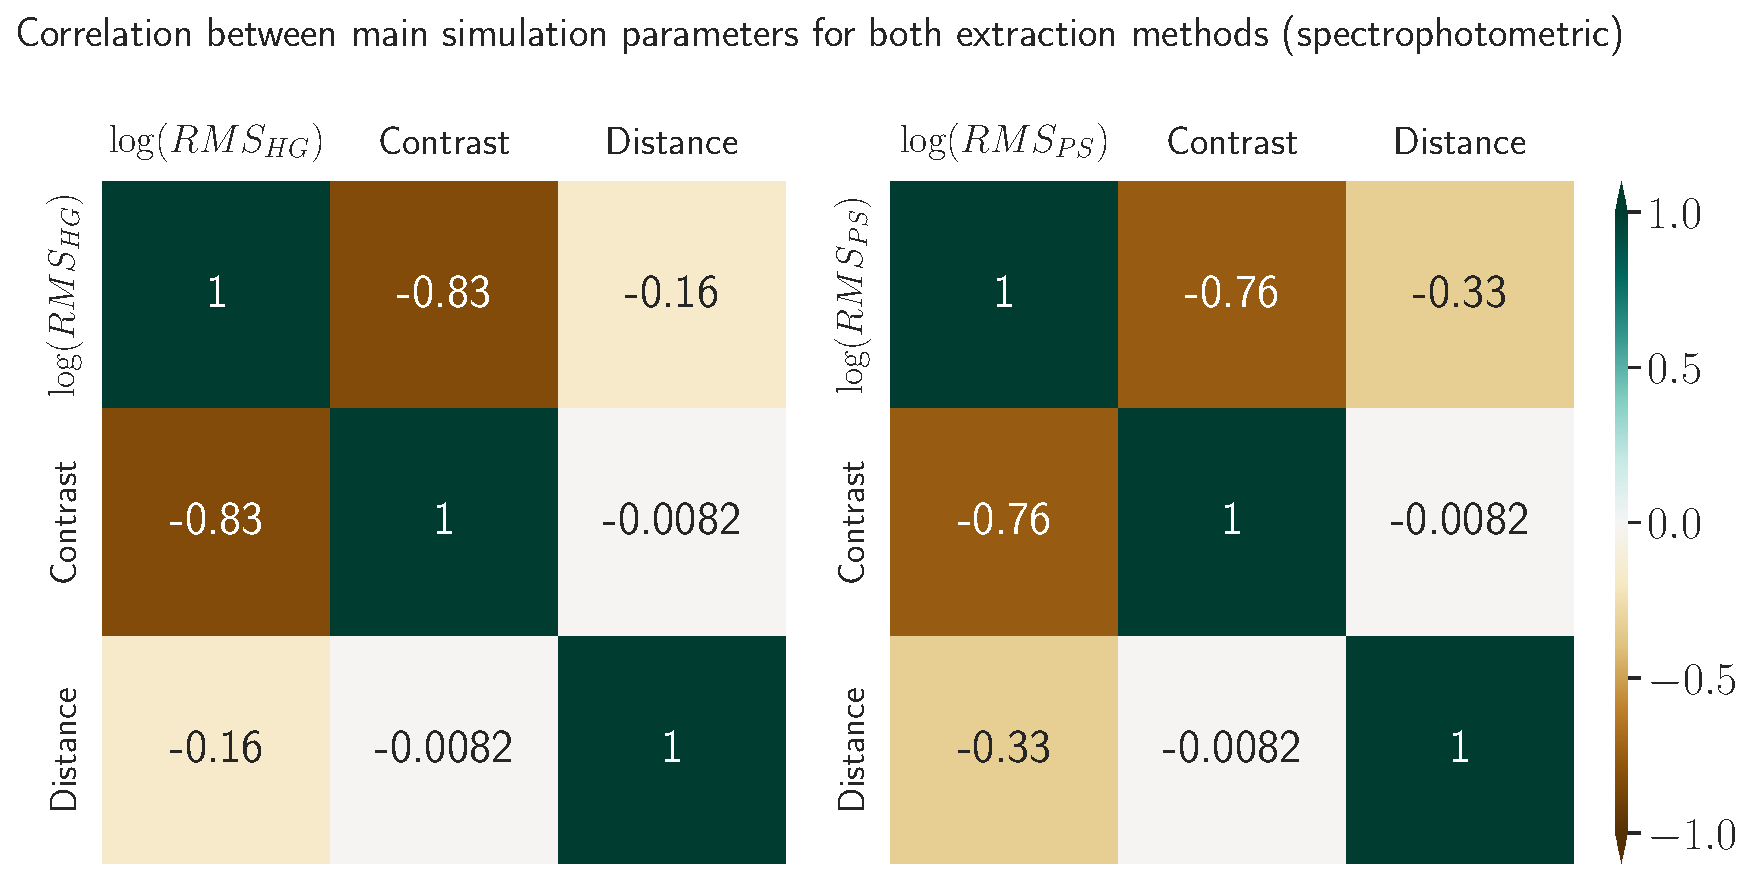
\includegraphics[width=\textwidth]{../figures/08_simu/corrheatmap_simu_params_spectrophoto.pdf}
  \end{minipage}\hfill
  \begin{minipage}[c]{0.38\textwidth}
    \caption[Corrélation des paramètres de la
    simulation (spectrophotométrique).]{Carte des coefficients de corrélation de Pearson des
      paramètres principaux de la
    simulation dans l'étude spectrophotométrique. Nous mettons en évidences ici l'impact de la distance
    sur le RMS quasiment inexistant pour la méthode \hypergal, mais
    légèrement influente sur la méthode d'extraction simple. Le SNR
    reste le paramètre ayant le plus d'impact sur la précision d'extraction.}\label{fig:corrheatmap_simuparams_spectrophoto}
  \end{minipage}
\end{figure}


Passons maintenant à l'analyse de la distribution du RMS spectral.
La Figure~\ref{fig:simu_rms_snr_spectrophoto} illustre l'évolution du
RMS spectral en fonction du SNR, en considérant des intervalles
contenant la même quantité de simulations.
La première information ressortant clairement de ces résultats et
l'amélioration indiscutable obtenue avec la modélisation hyperspectrale
de la galaxie, quelque soit le SNR. Par ailleurs, La méthode d'extraction basique
semble clairement inutilisable spectrophotométriquement sur l'ensemble
de la simulation, ne descendant sous les $10\%$ de RMS qu'à partir d'un
SNR$\approx100$.

La modélisation de scène quant à elle
approche un RMS$\approx10\%$ à partir d'un SNR$\approx40$, et
descend sous les $5\%$ vers un SNR$\approx100$. 

Nous montrons également la distribution des 3 permiers quartiles du
rapport $\frac{RMS_{PS}}{RMS_{HG}}$, et nous pouvons visualiser une
amélioration significative (environ un facteur $10$) entre les deux
méthodes quelque soit l'intervalle de SNR considéré. 

\begin{figure}[ht]
  \centering
  \makebox[\textwidth][c]{\includegraphics[width=0.9\textwidth]{../figures/08_simu/simu_rms_snr_spectrophoto.png}}%
  \caption[Distribution du RMS spectral en fonction du SNR.]{Distribution du RMS spectral en fonction du SNR  sur l'intervalle [$4000$,$8000$]\AA. Les
    distributions sont présentées en boîtes, dont les 3 barres
    centrales représentent les 3 quartiles ($25\%$, médiane et $50\%$). Nous illustrons ici une
    distribution de RMS spectral pour chacune des deux méthodes
    d'extraction et pour différents intervalles de SNR, chacun comptabilisant le
    même nombre de simulation. Nous montrons \emph{en haut} le RMS en $\%$
    en fonction du SNR. Les traits en pointillés indiquent les niveaux à
    $1\%$, $5\%$ et $10\%$. \emph{En bas} nous montrons le rapport
    $\frac{RMS_{PS}}{RMS_{HG}}$ pour illustrer l'amélioration apportée par
    \hypergal. Nous ne montrons que la boîte représentant les 3 quartiles de
    chaque distribution pour plus de clareté visuelle. Le trait en
    pointillés rouge indique un rapport de $1$}
  \label{fig:simu_rms_snr_spectrophoto}
\end{figure}

La Figure~\ref{fig:simu_rms_dist_spectrophoto} présente la même analyse,
cette fois ci en fonction d'intervalles de distance apparente entre la
galaxie hôte et la supernova. Comme attendu à partir de la matrice de
corrélation présentée précédemment, les distributions en RMS spectral
obtenues avec \hypergal\ n'indiquent aucune corrélation avec la
distance. La méthode d'extraction simple en revanche montre une
forte dégradation lorsque la distance est inférieur à $4\arcsec$, et
rejoint les performances d'\hypergal\ au dessus.

\begin{figure}[ht]
  \centering
  \makebox[\textwidth][c]{\includegraphics[width=0.9\textwidth]{../figures/08_simu/simu_rms_dist_spectrophoto.png}}%
  \caption[Distribution du RMS spectral en fonction de la distance
  hôte/SN.]{Distribution du RMS spectral en fonction du de la distance
    hôte/SN en arcsec sur l'intervalle [$4000$,$8000$]\AA. Les
    distributions sont présentées en boîtes, dont les 3 barres
    centrales représentent les 3 quartiles ($25\%$, médiane et $50\%$). Nous illustrons ici une
    distribution de RMS spectral pour chacune des deux méthodes
    d'extraction et pour différents intervalles de distances, chacun comptabilisant le
    même nombre de simulation. Nous montrons \emph{en haut} le RMS en $\%$
    en fonction de la distance. Les traits en pointillés indiquent les niveaux à
    $1\%$, $5\%$ et $10\%$. \emph{En bas} nous montrons le rapport
    $\frac{RMS_{PS}}{RMS_{HG}}$ pour illustrer l'amélioration apportée par
    \hypergal. Nous ne montrons que la boîte représentant les 3 quartiles de
    chaque distribution pour plus de clareté visuelle. Le trait en
    pointillés rouge indique un rapport de $1$}
  \label{fig:simu_rms_dist_spectrophoto}
\end{figure}

Quelque soit l'angle d'étude de la précision d'extraction photométrique,
la méthode incluant la modélisation hyperspectrale de la galaxie hôte
démontre une nette amélioration en comparaison avec une extraction
basique comme celle proposée par \pysedm.

Nous observons cependant que même le RMS spectral obtenu avec \hypergal
ne permet pas d'étude scientifique
spectrophotométrique avec la SEDm.

Cet instrument, tout comme ce pipeline, ne sont heureusement pas conçus à
cet effet mais à la classification des supernovae observées.

Ce procédé utilise la structure du spectre au travers des raies
d'absorptions/émissions caractéristiques de l'objet observé. La
classification va donc se baser sur les corrélations entre le spectre
extrait et une base de modèle dont la classification est a priori
connue. En ce sens, nous avons choisi d'analyser le RMS spectral en
retirant le continuum des spectres extraits, à l'instar de ce qui est
effectué par \pkg{SNID} \citep{BlondinSNID}.

\clearpage
\subsection{Précision avec correction de continuum}
% \label{ssec:xxx}

Afin de faire en sorte que le RMS spectral sonde la structure du spectre
extrait, indépendamment de l'amplitude relative avec le spectre de la
simulation, nous divisons les deux spectres par leur continuum
respectif. Bien que \pkg{SNID} utilise un polynome 
d'ordre $13$ pour déterminer ce continuum, nous préférons procéder à
cet ajustement avec un polynome
d'ordre $5$ afin d'éviter un potentiel sur-ajustement de certaines
caractéristiques des spectres.

Nous illustrons cette correction dans la
Figure~\ref{fig:continuumcorrection_ex}, où nous montrons la comparaison
entre un spectre extrait et celui simulé, avant et après division du
continuum. Nous pouvons visualiser dans cet exemple un effet de couleur
lors de l'extraction menant à un RMS spectral spectrophotométrique de
plus de $33\%$. En corrigeant par le continuum, on remarque que toutes
les structures du spectres sont nettement extrait par \hypergal, et
le RMS spectral tombe à $6\%$.

\begin{figure}[ht]
  \centering
  \makebox[\textwidth][c]{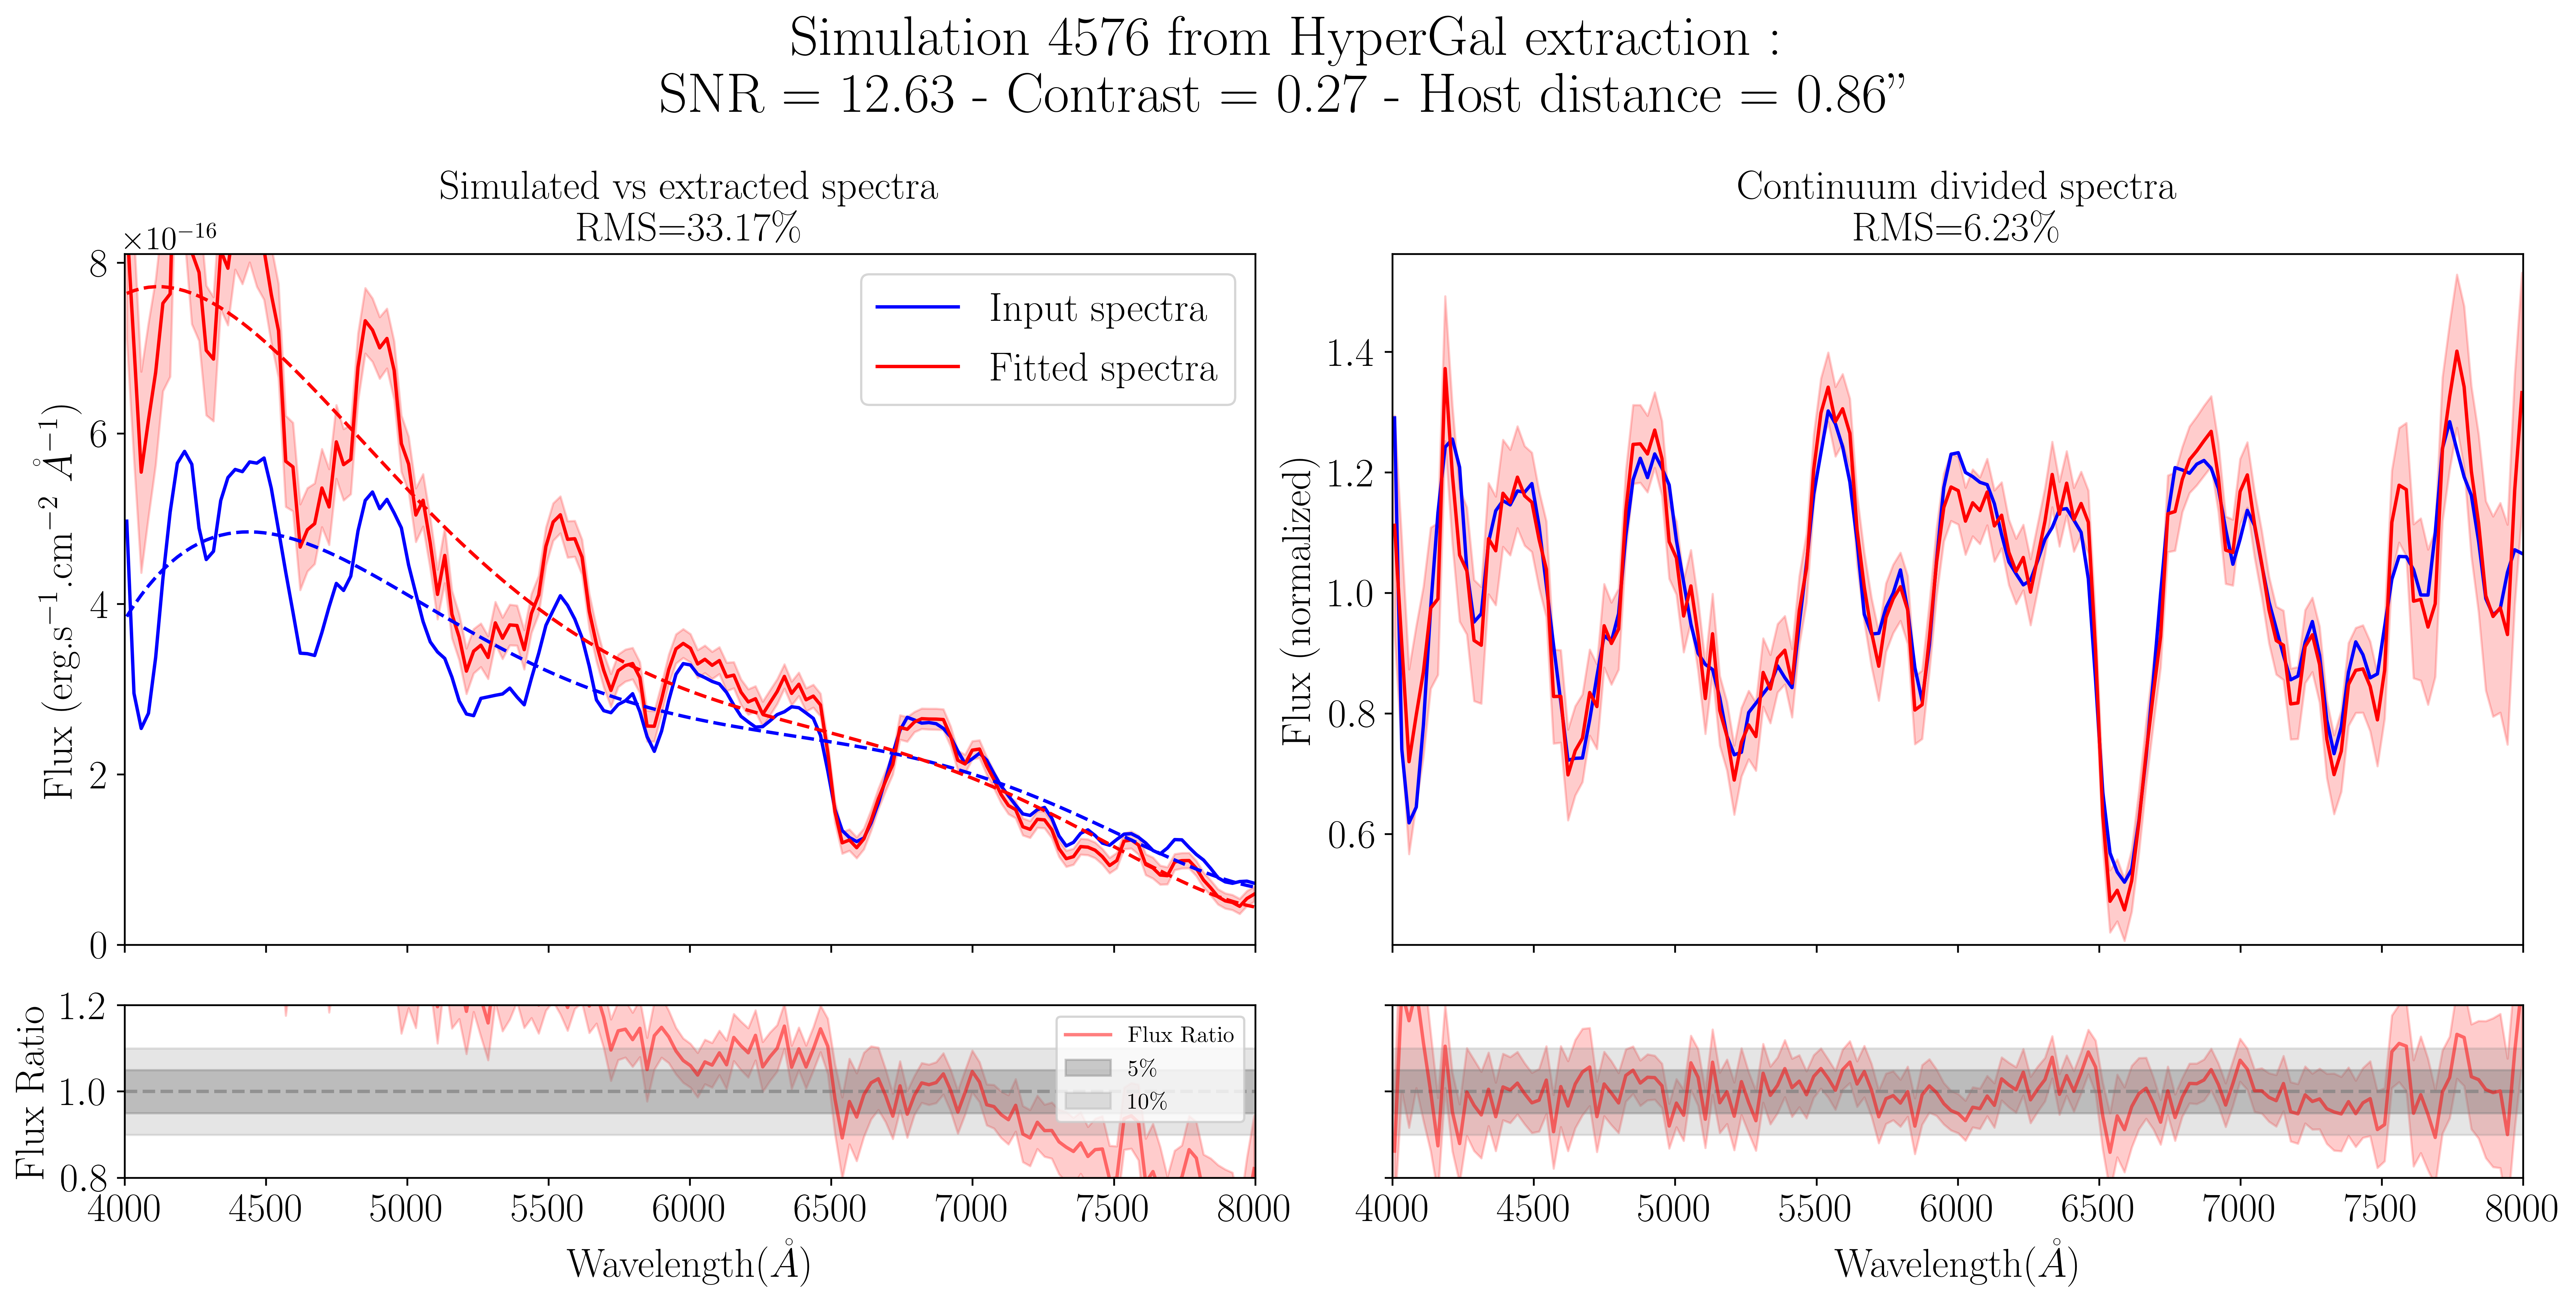
\includegraphics[width=1.2\textwidth]{../figures/08_simu/continuumcorrection_ex.png}}%
  \caption[Exemple de RMS spectral pour une simulation après correction
  du continuum.]{Exemple de RMS spectral pour une simulation après
    correction du continuum. Nous renseignons dans cet exemple les
    caractéristiques de la simulation, où nous avons un SNR de $12.6$,
    et une distance hôte/SN de $0\farcs86$. \emph{À gauche} nous
    montrons la comparaison du spectre simulé (en bleu) et du spectre
    extrait par \hypergal\ (en rouge), ainsi que le rapport entre les flux. Nous observons un effet de
    couleur intense dégradant fortement le RMS spectrophotométrique sur
    l'intervalle [$4000$,$8000$]\AA, atteignant plus de $33\%$. Les
    courbes en pointillés représentent le continuum ajusté avec un
    polynome d'ordre $5$. \emph{À droite} est présenté les mêmes
    spectres mais cette fois ci après division par le continuum. On peut
    voir que la
    structure du spectre simulé est très bien retrouvé, et cette
    correction ramène le RMS spectral à $\approx6\%$.}
  \label{fig:continuumcorrection_ex}
\end{figure}

Comme pour le cas spectrophotométrique, nous montrons dans la
Figure~\ref{fig:corrheatmap_simuparams} la carte des corrélations entre
les RMS(après division par le continuum) obtenus avec deux méthodes d'extraction et les différents paramètres de
la simulation. On remarque cette fois ci que la distance galaxie/SN
seule ne présente aucune corrélation avec le RMS spectral obtenu lorsque
l'on marginalise sur le SNR. La corrélation entre le RMS spectral et le
SNR est très fort, $-0.93$ pour la méthode \hypergal, et $-0.83$ pour
l'extraction simple. Nous pouvons raisonnablement en conclure que si l'objectif
est une classification, et donc la capacité 
d'extraction des caractéristiques du spectre, alors la connaissance du rapport signal sur
bruit est suffisante pour estimer la qualité de l'extraction, et ce
indépendamment de la distance entre la SN et sa galaxie hôte.
 
\begin{figure}[ht]
  \begin{minipage}[c]{0.6\textwidth}
    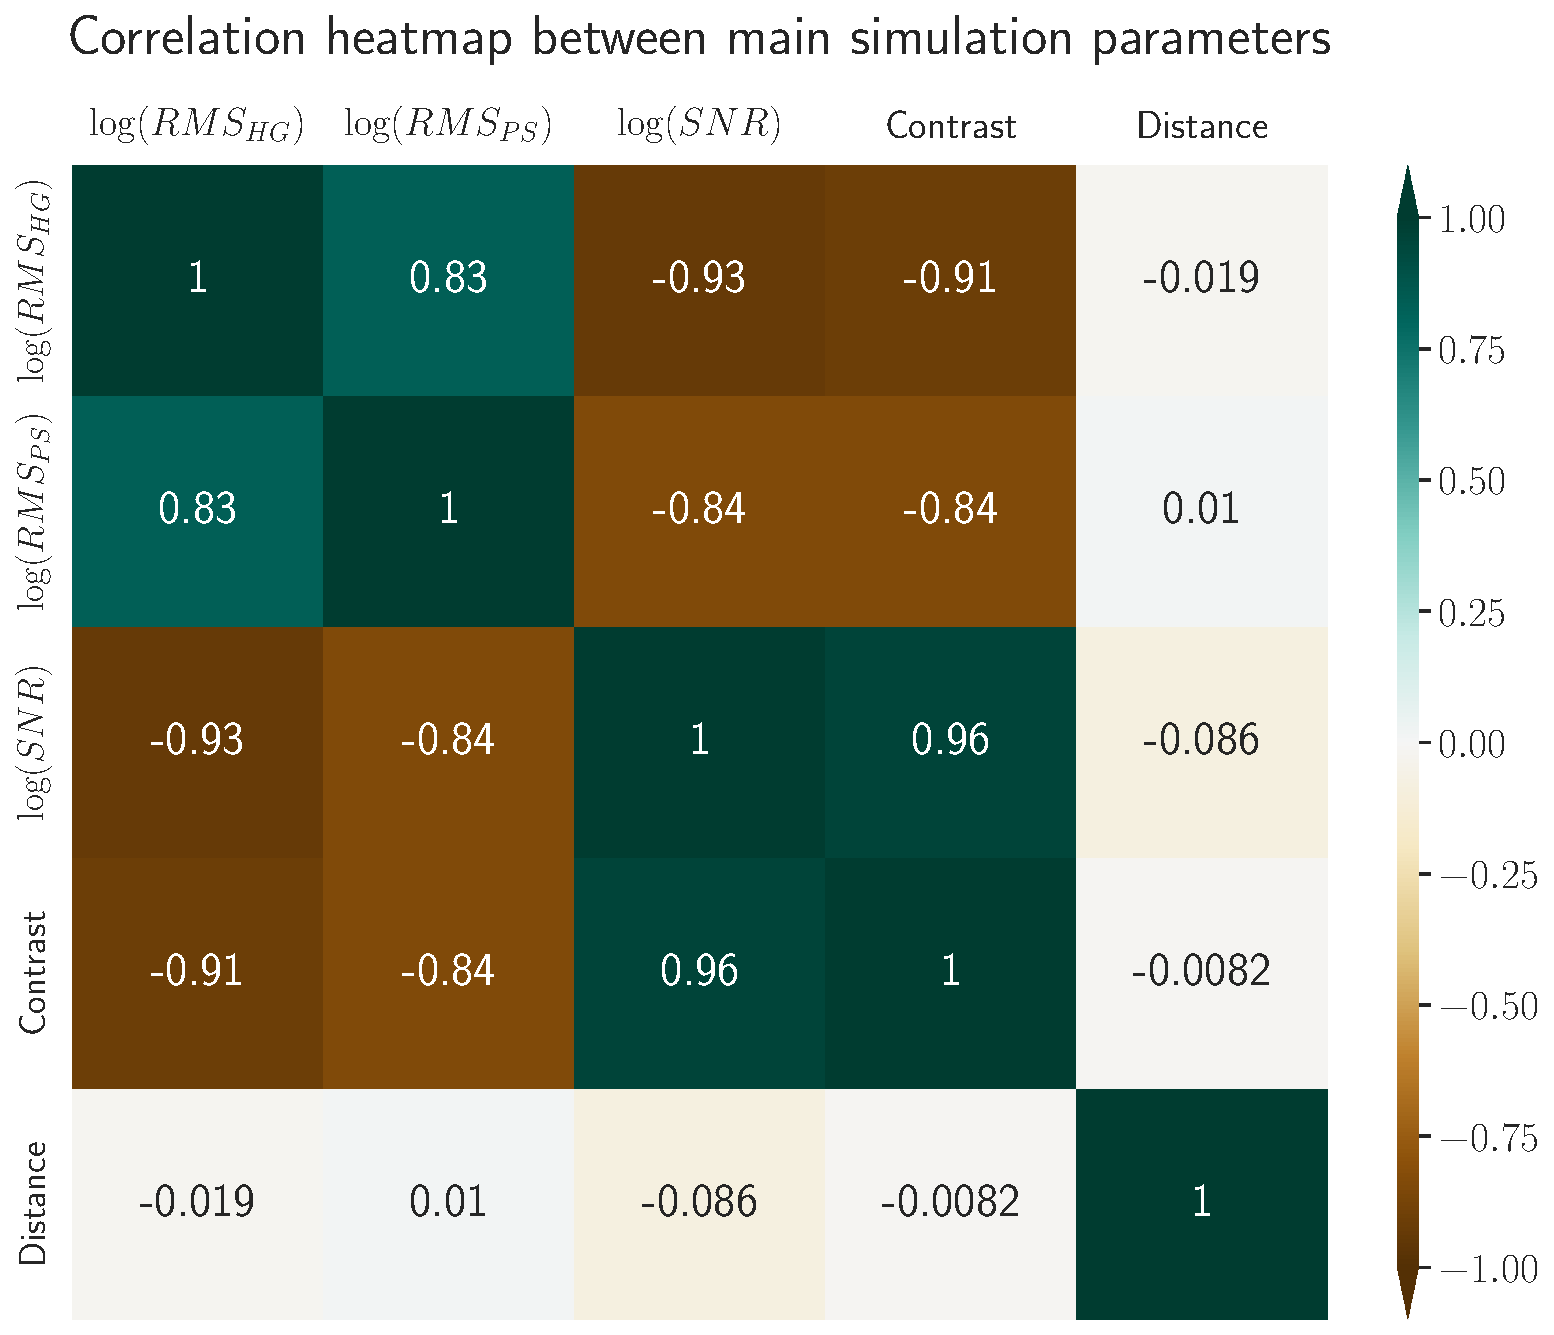
\includegraphics[width=\textwidth]{../figures/08_simu/corrheatmap_simu_params.pdf}
  \end{minipage}\hfill
  \begin{minipage}[c]{0.38\textwidth}
    \caption[Corrélation des paramètres de la
    simulation (continuum corrigé).]{Carte des coefficients de corrélation de Pearson des
      paramètres principaux de la
    simulation après correction du continnuum. La distance n'a plus
    aucune influence sur le RMS quelque soit la méthode.}\label{fig:corrheatmap_simuparams}
  \end{minipage}
\end{figure}

Avec cette information, il n'est pas vraiment d'intérêt à étudier
l'évolution du RMS en fonction de la distance. Nous nous focalisons donc
sur les résultats en fonction du SNR. La
Figure~\ref{fig:simu_rms_snr_continuum_divided} présente ainsi la
distribution en RMS spectral obtenue, après division par le continuum, en fonction de différents
intervalles de SNR pour les deux méthodes d'extraction. Indépendamment
de leur précision relative, nous apercevons que les deux méthodes
obtiennent un RMS spectral $>25\%$ pour un SNR$<4$. Dans l'intervalle
$4<\text{SNR}<8$, \hypergal\ commence à se démarquer avec un RMS allant
de $10\%$ à $30\%$, présentant une amélioration médiane de $20\%$ par
rapport à l'autre méthode d'extraction.  Le RMS médian à $10\%$ est
atteint pour un SNR de $\approx10$, et de $5\%$ pour un SNR de
$20$. Toutes les simulations avec un $\text{SNR}>40$ ont un RMS spectral
$<5\%$, et le seuil des $2\%$ est franchi dans plus de $80\%$ des
extractions pour un $\text{SNR}>60$.

Par rapport à la méthode d'extraction simple, \hypergal\ présente une
amélioration médiane d'environ $20\%$ dès un SNR de $\approx5$, pour monter à
environ $50\%$ entre $10<\text{SNR}<30$, et revenir progressivement à une amélioration
médiane de l'ordre de $20\%$ jusqu'aux derniers intervalles de SNR
étudiés ($>100$).

\begin{figure}[ht]
  \centering
  \makebox[\textwidth][c]{\includegraphics[width=1.\textwidth]{../figures/08_simu/simu_rms_snr_continuum_divided.png}}%
  \caption[Distribution du RMS spectral en fonction du SNR après
  correction du continuum.]{Distribution du RMS spectral en fonction du SNR après
    correction du continuum sur l'intervalle [$4000$,$8000$]\AA. Les
    distributions sont présentées en boîtes, dont les 3 barres
    centrales représentent les 3 quartiles ($25\%$, médiane et $50\%$). Nous illustrons ici une
    distribution de RMS spectral pour chacune des deux méthodes
    d'extraction et pour différents intervalles de SNR, chacun comptabilisant le
    même nombre de simulation. Nous montrons \emph{en haut} le RMS en $\%$
    en fonction du SNR. Les traits en pointillés indiquent les niveaux à
    $1\%$, $5\%$ et $10\%$. \emph{En bas} nous montrons le rapport
    $\frac{RMS_{PS}}{RMS_{HG}}$ pour illustrer l'amélioration apportée par
    \hypergal. Nous ne montrons que la boîte représentant les 3 quartiles de
    chaque distribution pour plus de clareté visuelle. Le trait en
    pointillés rouge indique un rapport de $1$.}
  \label{fig:simu_rms_snr_continuum_divided}
\end{figure}
%\begin{figure}[ht]
%  \centering
%  \makebox[\textwidth][c]{\includegraphics[width=1.\textwidth]{../figures/08_simu/simu_rms_dist_continuum_divided.png}}%
%  \caption[]{}
%  \label{fig:simu_rms_dist_continuum_divided}
%\end{figure}

\clearpage
\subsection{Efficacité de classification}\label{ssec:typingsimu}

La dernière analyse de nos simulations, et la plus importante dans le
cadre de la SEDm, est celle de l'efficacité d'\hypergal\ à classifier
les supernovae simulées.

Nous avons pour cela utilisé le même classifieur que ZTF, c'est à dire
\pkg{SNID}. Les critères de confiance que nous accordons pour la classification
sont cependant légèrement plus restreints, ayant régulièrement observé
des faux positifs dans les figures de contrôle du pipeline \pysedm. Nous
choisissons de fixer le r$lap$ minimal à r$lap_{min}=6$ pour le modèle
ajustant le mieux le spectre extrait. Par ailleurs, pour valider une
classification au moins $50\%$ des $10$ meilleurs modèles doivent être
du même type que le premier. Si un seul des critères ci-dessus n'est pas
respecté, alors nous classifions le spectre comme étant incertain.\\

Nous montrons dans la Figure~\ref{fig:typingimprove_snr} les résultats
de la classification obtenue avec \hypergal\ pour les $5000$
simulations, ainsi que l'amélioration par rapport à la méthode
d'extraction simple. Comme attendu avec l'étude du RMS spectral, il
semble illusoire d'espérer une classification de confiance lorsque le
SNR est inférieur à $4$. Une amélioration notable est visible dans
l'intervalle de $4<\text{SNR}\leq8$ pour les supernovae de type Ia,
\hypergal\ classifiant correctement $80\%$ d'entre elles. Cela
s'explique par le grand nombre de caractéristiques du spectre de ce type
de supernova, facilitant la classification. Les types Ibc et types II en
revanche ne sont retrouvés qu'à $25\%$ et $30\%$ respectivement, certainement parce que
ces spectres sont pauvrement structurés.

Le succès de classification monte ensuite entre $8<\text{SNR}\leq13$ à près de $95\%$ pour les Ia
, $88\%$ pour les types  Ibc et $57\%$ pour les types II.

Plus de $99\%$ des types Ia sont correctement classifiées à partir d'un
SNR de $13$, et plus de $96\%$ des toutes les supernovae sont
correctement classifiées pour un SNR supérieur à $30$.

L'amélioration vis à vis de la méthode d'extraction simple est
clairement identifiée, avec $33\%$ de Ia en plus entre $4<\text{SNR}\leq8$,
$27\%$ entre $8<\text{SNR}\leq13$, $15\%$ entre $13<\text{SNR}\leq20$ et
$9\%$ entre $20<\text{SNR}\leq30$. Au delà l'amélioration est marginale,
pour les Ia, mais reste de $19\%$ et $14\%$ pour les Ibc
et II respectivement entre $30<\text{SNR}\leq45$. Nous n'observons plus d'amélioration
notable lorsque le SNR est plus grand que
$45$.

Nous pouvons en déduire qu'\hypergal\ améliore drastiquement la
classification des supernovae lorsque le SNR est compris entre $4$ et
$45$, avec une zone optimale entre $8$ et $30$.

\begin{figure}[ht]
  \centering
  \makebox[\textwidth][c]{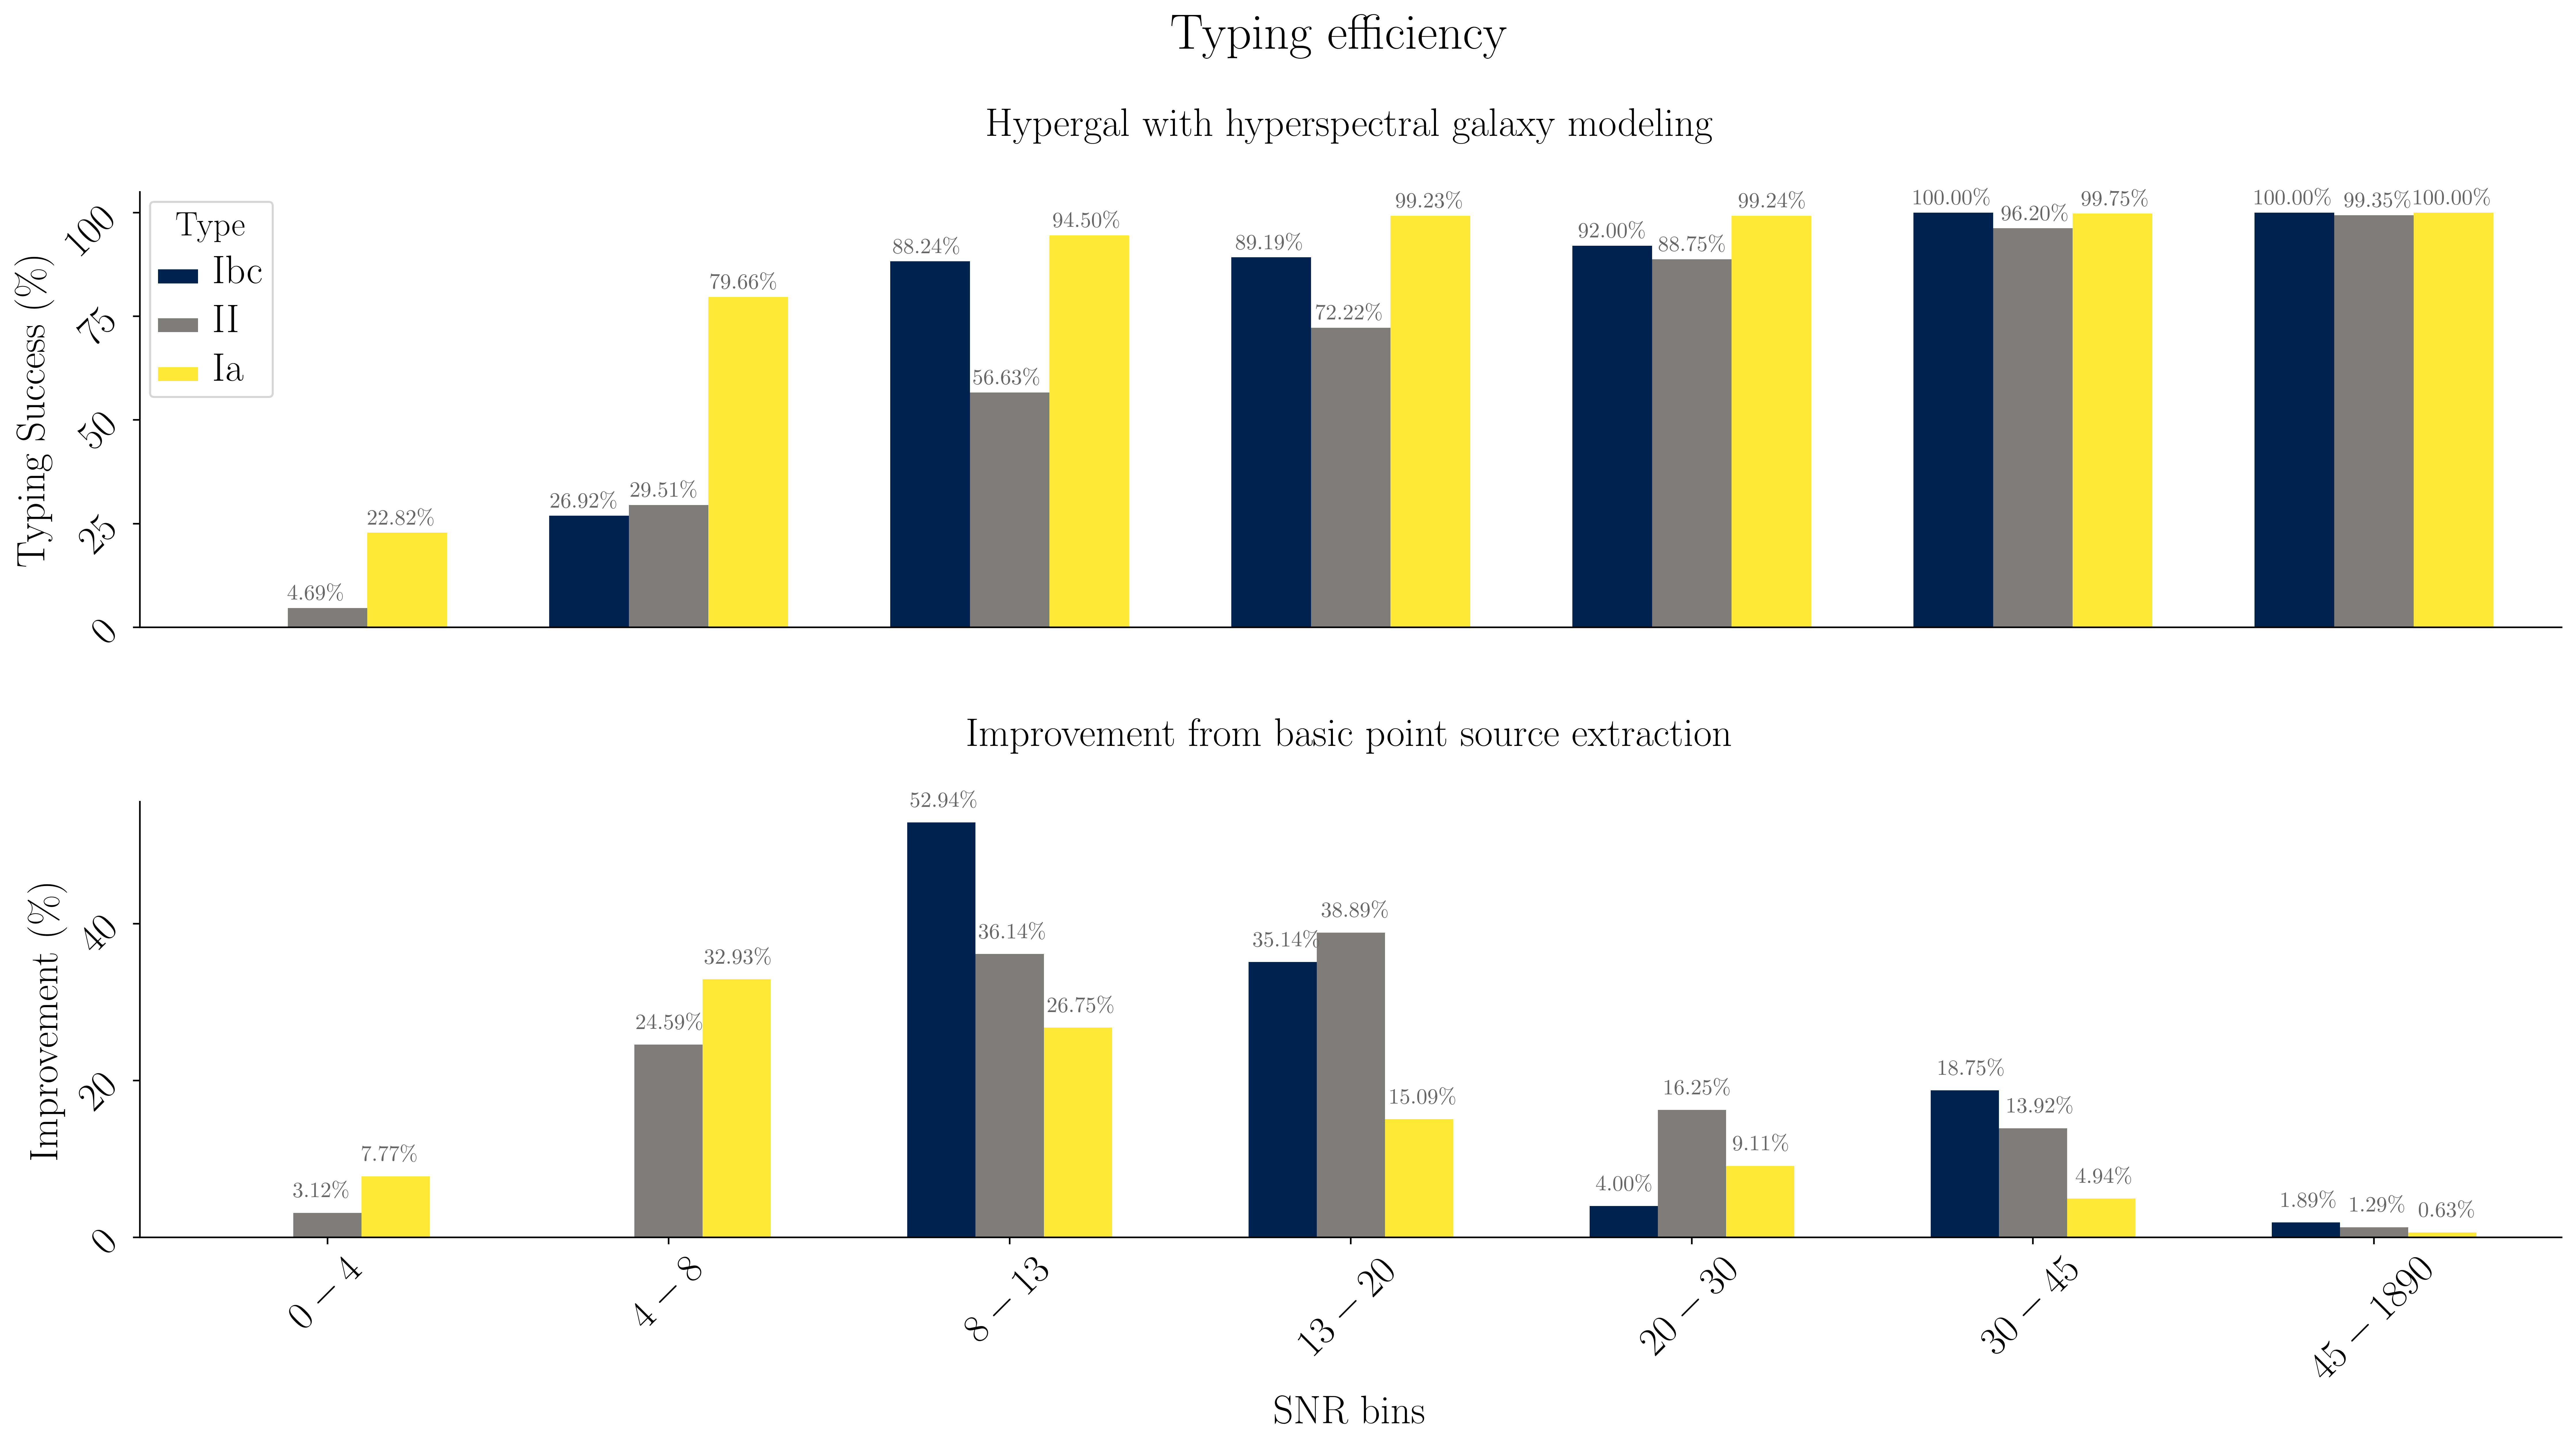
\includegraphics[width=1.2\textwidth]{../figures/08_simu/typingimprove_snr.png}}%
  \caption[Efficacité de classification des simulations.]{Efficacité de
    classification des simulations. \emph{En haut} nous montrons le pourcentage
  de classification réussie avec \hypergal\ pour chaque type de
  supernova et différents intervalles de SNR. Nous avons concaténé les $4$
  derniers intervalles de SNR car les résultats ne varient plus ou très
  peu au delà d'un SNR de $45$. \emph{En bas} nous montrons
  l'amélioration de classification par rapport à la méthode d'extraction
simple. }
  \label{fig:typingimprove_snr}
\end{figure}

Nous examinons par ailleurs le taux de faux positifs pour les supernovae
de type Ia, pouvant mener à une contamination des analyses cosmologiques
si non pris en compte. La Figure~\ref{fig:falsepositivesIa} montre ainsi
que pour l'intervalle $4<\text{SNR}\leq8$, malgré les $80\%$ de
classification corrects des Ia et l'amélioration de $33\%$ par rapport à
l'autre méthode d'extraction, nous avons près de $9\%$ de faux
positifs. Ce pourcentage diminue progressivement à environ $7\%$ entre
$8<\text{SNR}\leq13$, puis $5.5\%$ entre $13<\text{SNR}\leq20$ en enfin
environ $2.5\%$ pour un SNR entre $20$ et $45$. Au delà
d'un SNR de $45$, aucun faux positif n'est comptabilisé, autrement dit
toutes les classifications Ia sont effectivement des Ia.

À titre comparatif, la méthode d'extraction simple génère $12\%$ de faux
positifs entre  $8<\text{SNR}\leq13$ puis oscille entre $6.5\%$ et
$8.5\%$ dans l'intervalle $13<\text{SNR}\leq45$.

\begin{figure}[ht]
  \centering
  \makebox[\textwidth][c]{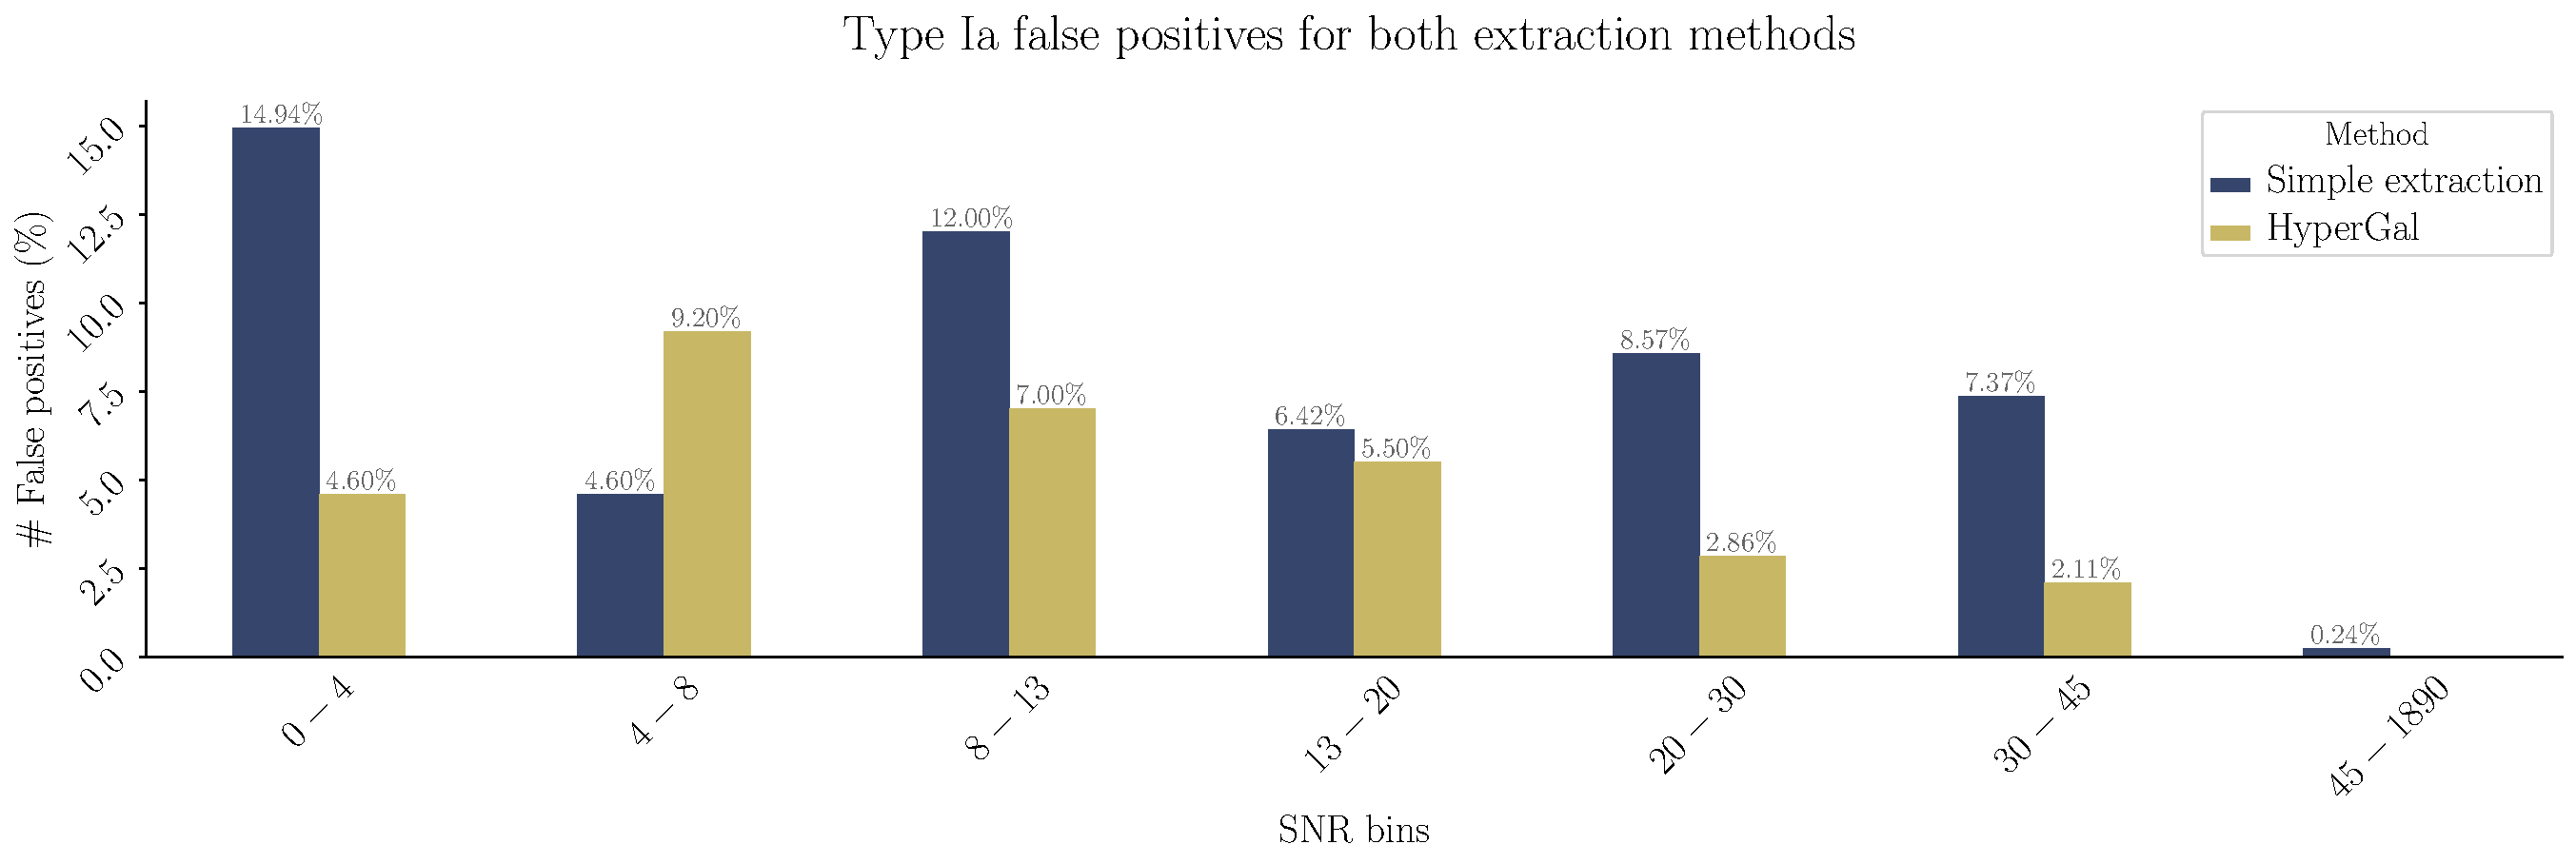
\includegraphics[width=1.2\textwidth]{../figures/08_simu/falsepositivesIa.pdf}}%
  \caption[Taux de faux positifs dans la classification des SNeIa.]{Taux de
    faux positifs dans la classification des SNeIa pour les deux
    méthodes d'extraction, en fonction du SNR. Le code couleur
    correspond aux deux méthodes d'extraction.}
  \label{fig:falsepositivesIa}
\end{figure}

Ces résultats illustrent ainsi une forte robustesse d'\hypergal\ à
classifier les supernovae et notamment les SNeIa à partir d'un
SNR$\approx10$, et surtout une amélioration conséquente vis à vis de
l'ancienne méthode d'extraction, sans la modélisation hyperspectrale de
la galaxie hôte. 

\bibliographystyle{../main/aa_url2}
\bibliography{99_references}
\end{document}

%%% Local Variables:
%%% mode: latex
%%% TeX-master: t
%%% End:
